% Kuramoto_thesis.tex
% ーーーーーーーーーーーーーーーーーーーーーーーーーーーーーーー

\documentclass[a4paper,12pt]{article_vdlab_sotsuron}
\pagestyle{plain}

\usepackage{setspace}
\usepackage{graphicx}
\usepackage{amsmath,amssymb}
\usepackage{colortbl}
\usepackage{comment}
% \usepackage{pdfpages}
% \usepackage{moreverb}
% \usepackage{multirow}

\begin{document}
%文字間隔を設定
\kanjiskip = .0pt plus 3pt minus 3pt
\xkanjiskip = .0pt plus 3pt minus 3pt
\small
\setstretch{1.5}

% ーーーーーーーーーーーーーーーーーーーーーーーーーーーーーーー

\begin{center}
  % 論文題目
  \jtitle{HILSにおけるモデル化誤差の影響評価}
  \etitle{Evaluation of Effects of Modeling error\\in Hardware-in-the-Loop Simulation}
\end{center}

%目次の表示
\tableofcontents

% ーーーーーーーーーーーーーーーーーーーーーーーーーーーーーーー

\newpage
\section{序論}
\subsection{タイヤとサスペンション}
自動車の「走る」「曲がる」「止まる」という基本的運動は,
車両と路面との唯一の接点であるタイヤ特性により成立している.
タイヤは自動車において唯一路面と接触する要素であり,この「走る」「曲がる」「止まる」という運動は,
全てこのタイヤと路面との間に発生する摩擦力によって実現している\cite{uno}.
そのため,タイヤは車両運動に直接影響を与える重要な要素といえる.
したがって,タイヤの特性を十分理解することで車両の運動特性を把握し,
その性能を十分に発揮させることができる\cite{nasu}.
タイヤはゴムの持つ材料特性などから強い非線形性を有しており,その力学特性を把握することは容易ではない.
一方,タイヤの状態に影響を及ぼす要因として,車体とタイヤを連結するサスペンション機構が挙げられる.
ホイールの上下ストロークに伴うアライメント変化,およびスプリングやダンパなどの特性は,
タイヤの接地状況に影響し,結果として車両の挙動にも影響を及ぼす.
従って,車両運動を評価する際には,タイヤの単体特性のみでなく,
サスペンションの特性を含めて評価を行うことが重要である\cite{shiiba}.

% ーーーーーーーーーーーーーーーーーーーーーーーーーーーーーーー
% Tire-suspension
%  ーーーーーーーーーーーーーーーーーーーーーーーーーーーーーーー
\vspace{20mm}
\begin{figure}[h]
  \centering
  \includegraphics[scale=0.7]{figure/suspension_tire.eps}
  \vspace{4mm}
   \caption{Tire-suspension Mechanism\cite{bmw}}
  \label{fig:tiresus}
\end{figure}
% ーーーーーーーーーーーーーーーーーーーーーーーーーーーーーーー

\newpage
\subsection{Hardware-in-the-Loop Simulation(HILS)システム}
Hardware-in-the-Loop Simulation (以下HILS)とは,評価対象のシステムの一部をハードウェアとして
シミュレーションのループ内に組込み,システム全体の特性を評価する手法である.
HILSはシステム全体のリアルタイム解析の結果に基づいて,ハードウェアへの入力を決定し,
ハードウェアの挙動を評価するとともに,システムの非線形特性を考慮したシステム全体の評価が実現できる.
シミュレーションにおいてパラメータ変更や様々な試験条件の設定できることから,
実機を用いた試験では再現が困難な条件での評価や,シミュレーションでは考慮できない実システムの非線形特性などを
考慮した評価が可能である.

これは従来の時刻歴シミュレーションと実機試験のそれぞれの欠点を補完するのようなものとなり,
シミュレーション精度の向上を図りながら,試験に必要なコストを抑え,試験の自由度を確保することができる.
このため,部品開発の一段階としてHILS試験を導入することで,精度と効率の両面において質の高い試験が可能となり,
開発の大幅な効率化が期待できる.\cite{yamaguchi}.

% ーーーーーーーーーーーーーーーーーーーーーーーーーーーーーーー
% HILS system
%  ーーーーーーーーーーーーーーーーーーーーーーーーーーーーーーー
\vspace{20mm}
\begin{figure}[h]
  \centering
  \includegraphics[scale=0.5]{figure/HILS_system.eps}
  \vspace{4mm}
   \caption{Concept of HILS System}
  \label{fig:HILSsystem}
\end{figure}
% ーーーーーーーーーーーーーーーーーーーーーーーーーーーーーーー

\newpage
\subsection{タイヤ-サスペンションHILSシステム}
先述のように車両運動特性を評価するためにはタイヤとサスペンションの特性を考慮して,
タイヤ-サスペンション系として複合的に評価する必要がある.
これらを評価する手法として,シミュレーションや実車走行試験がある.
しかし,タイヤは非線形特性を有しており,サスペンションはリンク配置などの複雑な構造から
正確に特性を把握することが難しい.
そのため,シミュレーションによる評価では,タイヤやサスペンションをモデル化することは困難である.
一方,実車走行試験による評価では,路面状況や天候などの影響により測定値のばらつきが大きいことや
同一条件で試験を行うことが困難である.
\par
そこで,当研究室においてタイヤ-サスペンション系の特性を評価するタイヤ-サスペンションHILSシステムを開発した.
このシステムではハードウェアに実車のタイヤ-サスペンション系を用いているため,
モデル化の困難であったタイヤ-サスペンション系の特性を考慮することができる.
また,路面状況など試験条件を一定にして試験を行うことが可能である.\cite{yamato}.
\par
開発されたタイヤ−サスペンション試験機は,サスペンションが取り付けられたている車体部分が固定されている.
そのため,車両運動解析で得られた車体と路面間の相対変位に基づいてモーションシステムを制御することで,実車のバウンシングを再現していた.
このHILSシステムでは解析モデルの精度が重要となることから,解析モデルとハードウェアの間に生じるモデル化誤差を把握することができれば,HILSシステムの再現性向上が期待できる.

% ーーーーーーーーーーーーーーーーーーーーーーーーーーーーーーー
% Tire-Suspension Testing Maschine
%  ーーーーーーーーーーーーーーーーーーーーーーーーーーーーーーー
\vspace{12mm}
\begin{figure}[h]
  \centering
  \includegraphics[scale=0.7]{figure/tire-suspension-machine.eps}
  \vspace{4mm}
   \caption{Tire-Suspension Testing Maschine}
  \label{fig:tiresusmachine}
\end{figure}
% ーーーーーーーーーーーーーーーーーーーーーーーーーーーーーーー

\newpage
\subsection{研究目的}
先述したとおり,HILSシステムは解析モデルの計算結果に基づいてハードウェアへの入力を決定し,システム全体の挙動を再現する.
そのため,解析モデルの精度はHILSシステムの再現性に影響を及ぼす.
そこで本研究では,HILSシステムにおけるモデル化誤差の影響を評価することを目的として,自動車のタイヤ-サスペンション系の上下挙動を模擬したHILS試験機を新たに開発しモデル化誤差がHILSシステムに及ぼす影響を評価した.
開発した試験機を用いてHILSシステムを構築し,解析モデルの計算結果とハードウェアの計測結果を比較することで,上下変位の解析結果を確認した.
また,モデル化誤差を変更してHILSシステムの上下変位を比較することで,モデル化誤差がHILSシステムの再現性に及ぼす影響を評価した.


\newpage
\section{HILSシステムの構成}
ここでは,本研究で新たに開発したHILSシステムについて説明する.
\subsection{システムの概要}
HILSシステムの概要を図\ref{fig:overviewhils}に示す.
このシステムは,ソフトウェア部である上下変位計算やシステム制御を行うPC,ハードウェア部であるHILS試験機やアクチュエータから構成されている.
本システムではHILS試験機において計測されたダンパの減衰力を用いて
リアルタイムに上下変位計算を行い,計算結果に基づきアクチュエータへの入力を決定し,HILS試験機の上下挙動を模擬するシステムである.

% % ーーーーーーーーーーーーーーーーーーーーーーーーーーーーーーー
% % Overview of HILS system
% %  ーーーーーーーーーーーーーーーーーーーーーーーーーーーーーーー
 \vspace{24mm}
\begin{figure}[h]
  \centering
  \includegraphics[height=80mm]{figure/hils_overview.eps}
  \vspace{4mm}
   \caption{Overview of HILS System}
  \label{fig:overviewhils}
\end{figure}
% % ーーーーーーーーーーーーーーーーーーーーーーーーーーーーーーー

\newpage
\subsection{ソフトウェア部}
本節では本研究において構築したHILS システムの解析環境について説明する.
HILS ではハードウェア側の時間変化に合わせて解析を行う必要があるため,リアルタイム解析を行う必要がある.
リアルタイム解析では,他のプログラムからの割込み要求の影響を受けず,
規定の時間間隔内での周期実行性が保証されたリアルタイムオペレーティングシステム(RTOS) が必要となる.

\subsubsection{dSPACEシステム}
本システムのソフトウェア部は,dSPACE社製の開発環境を利用し,リアルタイムシミュレーション環境を構築している.
この開発環境は,Controller Board,Real-Time Interface(RTI),Connector Panel,Control Deskで構成されており,システムの概要を図~\ref{fig:Configuration_of_software}~に示す.

\vspace*{10mm}
\begin{figure}[h]
  \begin{center}
     \includegraphics[scale=0.3]{figure/Configuration_of_software.eps}
     \vspace*{3mm}
     \caption{Configuration of Software}
     \label{fig:Configuration_of_software}
  \end{center}
\end{figure}

本システムでは,上下変位計算とハードウェア制御にdSPACE社製のController Board「DS1104 Controller Board」を使用している.
Controller Boardを図~\ref{fig:ds1104}~に,Connector Panelを図~\ref{fig:conpane}~に示す.
Controller Boardは,デジタル入出力用チャンネル,A/Dコンバータ用チャンネル,D/Aコンバータ用チャンネルを備えており,多くの用途に対応できる.
また,デジタルインクリメンタルエンコーダインターフェース用チャンネルによるエンコーダの計測や,シリアルインターフェースに対応しておりボーレート最大115200bpsのRS232通信が可能である.
Real-Time Interfaceは,dSPACE社製のハードウェアとMathWorks社製のソフトウェア「MATLAB/Simulink」の間のリンクとなるものである.
これにより,Simulinkモデルを用いてdSPACEシステムの入出力機器と信号処理を行うことができる.
また,MATLAB/Simulinkで作成されたモデルは,Simulink Corderにより,実時間で実行可能なCコードに変換され,Controller Board上で実行される.
このような開発環境を構築することで,実時間シミュレーションを行うHILSシステムを実現している.

\par
本試験機は,制御インターフェースとしてdSPACE社製のControl Deskを用いている.
「MATLAB/Simulink」と関連付けることで,試験条件の設定やハードウェアへの指令値,計測値,車両運動解析の結果をモニタリングできる.
また,リアルタイムで計測値や解析結果をグラフとして描画できる.図~\ref{fig:controldesk}~では指令値や計測値,上下変位計算の結果を表示したControl Deskの画面である.
なお,計測値はノイズを含むため,状況に応じてローパスフィルタをかけることが可能である.

% % ーーーーーーーーーーーーーーーーーーーーーーーーーーーーーーー
% % DS 1104
% %  ーーーーーーーーーーーーーーーーーーーーーーーーーーーーーーー
\vspace{12mm}
\begin{figure}[h]
    \begin{tabular}{cc}
      \begin{minipage}{0.5\hsize}
	\begin{center}
	  \includegraphics[height=30mm]{figure/ControllerBoard.eps}
	  \caption{Controller Borad~\cite{dspace}}
	  \label{fig:ds1104}
	\end{center}
      \end{minipage}

      \begin{minipage}{0.4\hsize}
	\begin{center}
	  \includegraphics[height=30mm]{figure/ConnectorPanel.eps}
	  \caption{Connector Panel~\cite{dspace}}
	  \label{fig:conpane}
	\end{center}
      \end{minipage}
    \end{tabular}
\end{figure}

% % % ーーーーーーーーーーーーーーーーーーーーーーーーーーーーーーー
% % % Control desk
% % %  ーーーーーーーーーーーーーーーーーーーーーーーーーーーーーーー
 \vspace{15mm}
\begin{figure}[h]
  \centering
  \includegraphics[height=70mm]{figure/ControlDesk.eps}
  \vspace{2mm}
%   \includegraphics[scale=0.6]{flatbelt.eps}
   \caption{Control Desk}
  \label{fig:controldesk}
\end{figure}
% ーーーーーーーーーーーーーーーーーーーーーーーーーーーーーーーー


\newpage
\subsubsection{上下変位計算}
このHILSシステムはサスペンション部分の上下挙動を模擬するため,時刻歴応答シミュレーションにより上下変位を計算している.計算に用いる解析モデルとして,上下2自由度モデルを用いた\cite{2dof}.
このモデルは車両の上下方向の運動の基本的な性質を理解するためにもっとも簡単な
2自由度ばね-マス系の一般的な解析手法が適用可能である.
このモデルを図~\ref{fig:2DOF}~に,諸元を表~\ref{tab:2DOF}~に示す.
運動方程式は式~(\ref{eq:2DOF_1})~,~(\ref{eq:2DOF_2})~ に示す.
また,このHILSシステムは入力$x_0$に対して計算した上下変位$x_2-x_1$に基づき,アクチュエータを制御している.


\vspace*{-10mm}
\begin{flalign}
\label{eq:2DOF_1}
& m_1\ddot{x_1}+k_1(x_1-x_0)+k_2(x_1-x_2)-f_c=0 \\
\label{eq:2DOF_2}
& m_2\ddot{x_2}+k_2(x_2-x_1)+f_c=0
\end{flalign}

\vspace{-2mm}
ここで,$m_2$はばね上質量,$m_1$はばね下質量,$k_2$はばね定数,$k_1$はタイヤの縦ばね剛性,$x_0$は路面変位,$x_1$はばね下変位,$x_2$はばね上変位である.
そして,$f_c$はHILS試験機で計測したダンパ力を用いる.



% ーーーーーーーーーーーーーーーーーーーーーーーーーーーーーーーー
%2dof Vehicel Model
% ーーーーーーーーーーーーーーーーーーーーーーーーーーーーーーー
\vspace{10mm}
\begin{figure}[h]
  \begin{minipage}{0.3\hsize}
     \begin{center}
      \includegraphics[height=35mm]{figure/model_2dof_f.eps}
	\vspace{2mm}
      \caption{2DOF Model}
      \label{fig:2DOF}
    \end{center}
  \end{minipage}
\begin{minipage}{0.65\hsize}
\makeatletter
\def\@captype{table}
\makeatother
  \begin{center}
   \caption{Parameter of 2DOF Model}
   \label{tab:2DOF}
   \begin{tabular}{cc}\hline
      Sprung Mass $m_2$ [kg] & 6.4  \\l
      Unsprung Mass $m_1$ [kg] & 1.5 \\
      Spring constant $k_2$ [N/m] & 405  \\
      Vertical spring stiffness $k_1$ [N/m] & 2200   \\ \hline
%       Damping coefficient $c_2$ [N/m] & 7   \\
%       Damping coefficient $c_1$ [N/m] & 150   \\ \hline
    \end{tabular}
   \end{center}
 \end{minipage}
\end{figure}
% ーーーーーーーーーーーーーーーーーーーーーーーーーーーーーーーー

\newpage
\subsubsection{ハードウェア制御}
ここでは,アクチュエータへの入力を算出する方法について説明する.
アクチュエータへの入力$\bar{x}_0$は,解析モデルを用いて計算した上下変位$x_2-x_1$に基づき決定する.
解析モデルは上下2自由度振動系であるのに対し,開発したHILS試験機はばね上が固定された1自由度振動系である.
2自由度振動系の上下変位$x_2-x_1$は,1自由度振動系の$-\bar{x}_1$に相当する.
そこでHILS試験機を1自由度振動系としてモデル化し,入力$\bar{x}_0$に対する上下変位$-\bar{x}_1$の逆伝達関数を考慮してアクチュエータへの入力を決定する必要がある.
このとき,逆モデルの計算を行うためダンパは線形とし,装置の周波数応答から$c_2$をパラメータ同定した.
ハードウェアのモデルを図~\ref{fig:1DOF}に,諸元を表~\ref{tab:1DOF}~に示す.
運動方程式は式~(\ref{eq:1DOF})~ に示す.
また,HILSシステムのブロック線図を図~\ref{fig:block_HILS}に示す.

\vspace*{-10mm}
\begin{flalign}
\label{eq:1DOF}
\ & m_1\ddot{\bar{x}}_1+c_2\dot{\bar{x}}_1+k_1(\bar{x}_1-\bar{x}_0)+k_2\bar{x}_1=0
\end{flalign}

\vspace{-2mm}
ここで,$m_1$はばね下質量 ,$m_2$はばね上質量,$k_1$はタイヤの縦ばね剛性,$k_2$はばね定数,$c_2$は減衰係数,$\bar{x}_0$はHILS試験機の路面部変位,$\bar{x}_1$はばね下部変位である.

% ーーーーーーーーーーーーーーーーーーーーーーーーーーーーーーーー
%1dof Vehicel Model
% ーーーーーーーーーーーーーーーーーーーーーーーーーーーーーーー
\vspace{10mm}
\begin{figure}[h]
  \begin{minipage}{0.3\hsize}
     \begin{center}
      \includegraphics[height=35mm]{figure/model_1dof.eps}
	\vspace{2mm}
      \caption{1DOF Model}
      \label{fig:1DOF}
    \end{center}
  \end{minipage}
\begin{minipage}{0.65\hsize}
\makeatletter
\def\@captype{table}
\makeatother
  \begin{center}
   \caption{Parameter of 1DOF Model}
   \label{tab:1DOF}
   \begin{tabular}{cc}\hline
      Unsprung Mass $m_1$ [kg] & 1.5  \\
      Vertical spring stiffness $k_1$ [N/m] & 2200  \\
      Spring constant $k_2$ [N/m] & 405   \\
      Damping coefficient $c_2$ [N/m] & 7   \\ \hline
    \end{tabular}
   \end{center}
 \end{minipage}
\end{figure}
% ーーーーーーーーーーーーーーーーーーーーーーーーーーーーーーーー
% % ーーーーーーーーーーーーーーーーーーーーーーーーーーーーーーー
% % Block diagram
% %  ーーーーーーーーーーーーーーーーーーーーーーーーーーーーーーー
 \vspace{8mm}
\begin{figure}[h]
  \centering
  \includegraphics[height=45mm]{figure/block_HILS.eps}
  \vspace{2mm}
   \caption{Block Diagram}
  \label{fig:block_HILS}
\end{figure}
% ーーーーーーーーーーーーーーーーーーーーーーーーーーーーーーーー

\newpage
\subsection{ハードウェア部}
\subsubsection{HILS試験機}
本研究で開発したHILS試験機を図~\ref{HILSmachine}に示す.
この装置は上下1自由度で路面部にアクチュエータを取り付けている.
自動車の車体をばね上で,タイヤ-サスペンション系をばね下とばね・ダンパで表現している.
\par
ソフトウェア部で計算したサスペンションストロークをばね上ばね下間の変位として実現している.
また,レーザ変位計とロードセルを用いて,サスペンションストロークとダンパ力を計測している.

%  ーーーーーーーーーーーーーーーーーーーーーーーーーーーーーーー
% Tire testing machine
%  ーーーーーーーーーーーーーーーーーーーーーーーーーーーーーーー
\vspace{24mm}
\begin{figure}[h]
  \begin{center}
  \includegraphics[height=80mm]{figure/HILS_machine_E.eps}
  \vspace{4mm}
   \caption{HILS Testing Machine}
  \label{HILSmachine}
  \end{center}
\end{figure}


\newpage
\subsubsection{アクチュエータ}
ここでは,アクチュエータとして用いるモータとその制御ユニットとして用いるモータドライバについて説明する.また,モータの制御方法について説明する.
\par
まず,本試験機に用いるモータは,maxon japan株式会社のECモータ「EC-max 40 283867」である.
モータの外観を図~\ref{fig:EC_motor}~に,仕様を表~\ref{tab:EC_motor}~に示す.
モータの先端には,ギアヘッドが取り付けられ,回転方向や角度を検出する電子部品としてエンコーダが取り付けられている.
使用するモータでは,maxon motor社製のプラネタリギアヘッド「GP 42 C 203126」とエンコーダ「HEDL 5540 110516」を取り付けている.
それぞれの諸元を表~\ref{tab:Gearhead}~,表~\ref{tab:Encoder}~に示す.

\vspace*{5mm}
\begin{figure}[h]
  \begin{minipage}{0.4\textwidth}
    \centering
      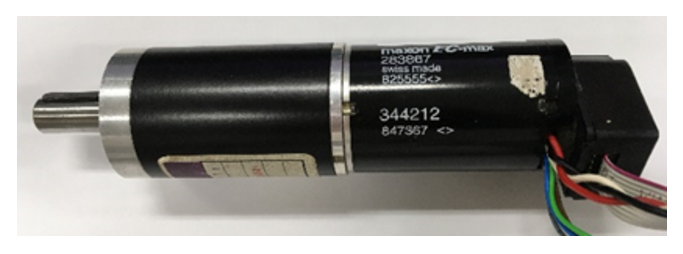
\includegraphics[height=20mm]{figure/ecmax40.eps}
      \vspace*{3mm}
      \caption{ECmax 40 283867}
      \label{fig:EC_motor}
  \end{minipage}
  \begin{minipage}{0.5\textwidth}
      \centering
	\makeatletter
	\def\@captype{table}
	\makeatother
	\caption{Specification of EC motor (283867)}
	\label{tab:EC_motor}
	  \begin{tabular}{cc}\hline
	    Parameter & Value \\\hline
	    Nominal output & 70 [W] \\
	    Nominal voltage & 24 [V] \\
	    Nominal speed & 8040 [rpm] \\
	    Max continuous Torque & 89.6 [mNm] \\
	    Max continuous current & 3.44 [A] \\
	    Torque constant & 28 [mNm/A] \\
	    Speed constant & 341 [rpm/V] \\\hline
	  \end{tabular}
  \end{minipage}
\end{figure}
\vspace*{10mm}
\begin{table}[h]
  \begin{center}
    \caption{Specification of Encoder (110516)}
    \label{tab:Encoder}
      \begin{tabular}{cc}\hline
      Parameter & Value \\\hline
      Encoder Resolution & 500 [count/rev] \\
      Max frequency & 100 [kHz] \\
      Allowable maximum speed & 12000 [rpm] \\\hline
    \end{tabular}
  \end{center}
\end{table}\vspace*{10mm}
\begin{table}[h]
  \begin{center}
    \caption{Specification of Gearhead (223084)}
    \label{tab:Gearhead}
    \begin{tabular}{cc}\hline
      Parameter & Value \\\hline
      Gear Ratio & 113:1 \\
      Rated speed & 8000 [rpm] \\
      Backlash & 1.0 [deg] \\
      Max continuous torque & 15 [Nm] \\\hline
    \end{tabular}
  \end{center}
\end{table}


\newpage

次に,モータドライバについて説明する.先ほどのモータの制御ユニットとしてmaxon motor社製のデジタル位置制御ユニット「EPOS2 70/10 375711」を使用した.
このモータドライバの外観を図~\ref{fig:Motor_driver}~に,仕様を表~\ref{tab:Motor_driver}~に示す.
EPOS2は,インクリメンタル・エンコーダ付きDCモータおよびEC(ブラシレス)モータを駆動可能なデジタル位置制御ユニットである.
CANopen,USB 2.3/3.0,RS232通信による通信を可能とし,Point to pointの位置制御,回転数制御,トルク制御を行うことができる.
EPOS2 70/10は,モジュール式のデジタル制御ユニットで,80〜700 Wまでのエンコーダ付きDCモータ,またはホールセンサ/エンコーダ付きブラシレスECモータに対応している.
本研究では,RS232通信を用いて位置指令を行い,「Position Mode」を用いて位置制御によりモータを制御している.
このモータドライバの電源電圧の供給には,図~\ref{fig:rs_150_24}~に示すMEAN WELL社のスイッチング電源「RS-150-24」を使用した.

% % ーーーーーーーーーーーーーーーーーーーーーーーーーーーーーーー
% % Step
% %  ーーーーーーーーーーーーーーーーーーーーーーーーーーーーーーー
\vspace{10mm}
\begin{figure}[h]
    \begin{tabular}{cc}
      \begin{minipage}{0.5\hsize}
	\centering
	  \includegraphics[height=40mm]{figure/EPOS2.eps}
	  \begin{center}
	  \vspace{2mm}
	  \caption{EPOS2 70/10 375711}\
	  \label{fig:Motor_driver}
	  \end{center}
	\end{minipage}
       \begin{minipage}{0.45\hsize}
	\centering
	  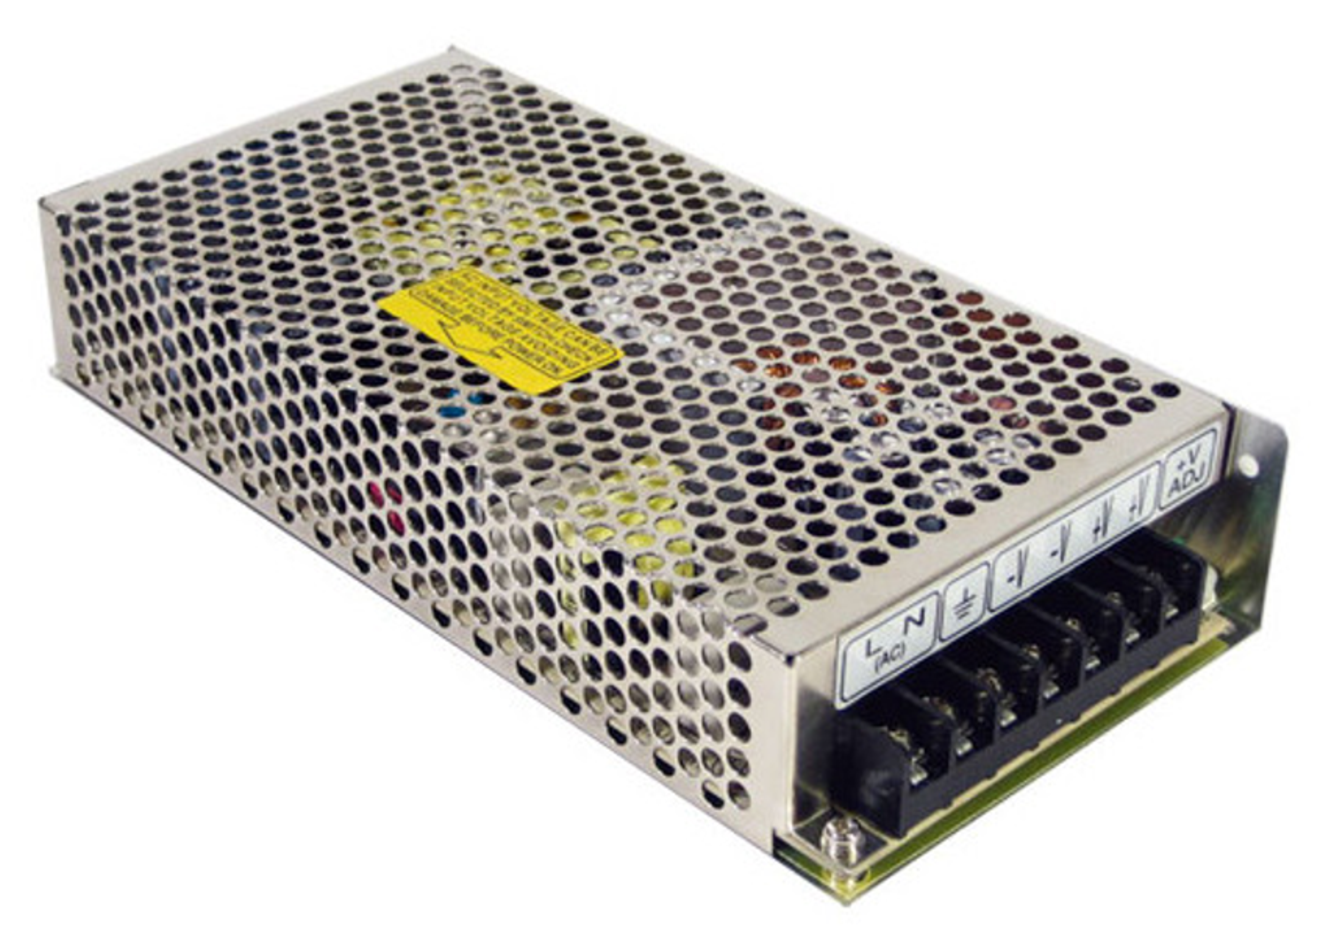
\includegraphics[height=40mm]{figure/rs_150_24.eps}
	  \begin{center}
	  \vspace{2mm}
	  \caption{RS-150-24}\
	  \label{fig:rs_150_24}
	  \end{center}
      \end{minipage}
    \end{tabular}
    \vspace{2mm}
\end{figure}


\vspace*{10mm}
\begin{table}[h]
  \begin{center}
    \caption{Specification of EPOS2 70/10 (375711)}
    \label{tab:Motor_driver}
    \begin{tabular}{cc}\hline
      Parameter & Value \\\hline
      power suppy voltage & 11-70 [VDC] \\
      Max output current & 25 [A] \\
      Max continuous current & 10 [A] \\
      Hall sensor & H1, H2, H3 \\
      Encoder & A, A$\setminus$, B, B$\setminus$, I, I$\setminus$(max. 5MHz)\\
      Analog Input & 2(differential, 12-bit, 0...+5 V)\\
      RS232 & RxD; TxD(max. 115200 bit/2) \\\hline
    \end{tabular}
  \end{center}
\end{table}


\newpage
また,maxon motor社製のグラフィカル・ユーザ・インターフェイス「EPOS Studio」を用いて使用するモータやエンコーダなどにモータドライバが適合するようシステム設定を行うことができる\cite{maxon}.
また,制御ゲインのオート・チューニング機能を用いて,電流,速度,位置の制御ゲインを自動的に調整している.
図~\ref{fig:studio}に「Position Mode」を用いる際の「EPOS Studio」の画面を示す.

\vspace*{10mm}
\begin{figure}[h]
  \begin{center}
    \includegraphics[height=75mm]{figure/EPOSStudio.eps}
     \vspace*{5mm}
     \caption{EPOS Studio (Position Mode)}
     \label{fig:studio}
  \end{center}
\end{figure}


\newpage
\subsubsection{計測器}
本試験ではダンパ力とサスペンションストロークを計測する.
ここでは計測に用いるロードセルとレーザ変位計について説明する.
\par
まず,ロードセルについて説明する.ダンパ力を計測するために東京測器研究所社製のTCLZ-20NAのロードセルを用いた.
ロードセルの外観を図~\ref{fig:loadcell}に示す.仕様について,表~\ref{tab:loadcell}~に示す.
このロードセルは引張圧縮両用型で,小型軽量・高精度な荷重計である.
ロードセルから出力された電圧は,東京測器研究所社製のデジタル指示計「TD-96A」を用いて換算する.
デジタル指示計の外観を図~\ref{fig:TD-96A}~に,仕様を表~\ref{tab:TD-96A}~に示す.
このデジタル指示器は,ひずみゲージ式変換器を用いて荷重,変位,圧力などを測定できる.
測定時は,デジタル指示器で初期設定を行い,測定値のモニタリングとデータの保存は,dSPACE社製の開発環境を利用している.
また,測定値は電圧値として$\pm{10}[V]$で出力しているため,それを$\pm{20}[N]$の力に換算する必要がある.換算式を式~(\ref{eq:loadcell})~に示す.

\vspace{-10mm}
\begin{eqnarray}
\label{eq:loadcell}
 &  Force [N] = \ Voltage \ [V]\times \frac{20}{10}
\end{eqnarray}
% ----------------------------------------------------------------------
\vspace{-8mm}
\begin{figure}[h]
\begin{tabular}{cc}
\begin{minipage}{0.45\textwidth}
    \centering
    \includegraphics[height=35mm]{figure/TCLZ-20NA.eps}
     \vspace{2mm}
     \caption{TCLZ-20NA}
     \label{fig:loadcell}
\end{minipage}
\begin{minipage}{0.45\hsize}
\centering
     \includegraphics[height=35mm]{figure/TD-96A.eps}
     \vspace{2mm}
     \caption{TD-96A}
     \label{fig:TD-96A}
\end{minipage}
\end{tabular}
\end{figure}

\vspace{1mm}
 \begin{quote}{\small
\begin{table}[htbp]
 \begin{center}
 \caption{Specification of TCLZ-20NA}
 \label{tab:loadcell}
 \begin{tabular}{crrc}\hline
    Parameter & \multicolumn{2}{c}{Value}&\\\hline
    Capacity & \multicolumn{2}{c}{20 N}&\\
    Overload Capacity & \multicolumn{2}{c}{30N}&\\
      & Ten.&Comp.\\
    Rated Output & +1248.7 & -1248.4 & $\mu$V/V \\
    Strain & +2497.3 & -2496.8 & $\times 10^{-6}$ $\epsilon$ \\
    Calibration Coefficient & 0.008009 & 0.008010 & N/1$\times 10^{-6}$ \\\hline
  \end{tabular}
 \end{center}
\end{table}
}\end{quote}

\vspace*{1mm}
 \begin{quote}{\small
\begin{table}[htbp]
 \begin{center}
 \caption{Specification of TD-96A}
  \label{tab:TD-96A}
    \begin{tabular}{ccc}\hline
      Parameter & Value \\\hline
      Measurement Point & 1 \\
      Measurement Range & $\pm$3 mV/V\\
      A/D Conversion Speed & 4000 Hz\\
      D/A Output & 0$\pm$1$\sim\pm$10 V, 4$\sim$20 mA\\
      Power supply & AC100 V 12 W, DC12$\sim$24 V 9 W \\\hline
  \end{tabular}
 \end{center}
\end{table}
}\end{quote}
% ----------------------------------------------------------------------

\newpage
次に,レーザ変位計について説明する.本試験ではサスペンションストロークを計測するために,ばね下の変位量を計測する.計測にはKEYENCE社製のレーザ変位計「IL-300」を用いた.
レーザ変位計の外観を図~\ref{IL-300}に示し,仕様を表~\ref{tab:IL-300}に示す.
このレーザ変位計を使用する際は,図~\ref{IL-1500}のアンプユニット「IL-1500」をレーザ変位計に接続する必要がある.
図~\ref{KZ-U3}のスイッチング電源「KZ-U3」を用いて,24Vをアンプユニットに供給している.
\par
測定時は,アンプユニットで初期設定を行い,測定値のモニタリングとデータの保存は,dSPACE社製の開発環境を利用している.
また,測定値は電圧値$\pm{5}[V]$として得られるため,それを距離に換算する必要がある.換算式を式~(\ref{eq:lazer})~に示す.

\vspace*{-2mm}
\begin{eqnarray}
\label{eq:lazer}
 & Displacement[mm] = Voltage\ [V]\times28
\end{eqnarray}

\vspace*{2mm}
\begin{figure}[htp]
  \begin{minipage}{0.3\hsize}
     \begin{center}
     \vspace*{5mm}
      \includegraphics[height=35mm]{figure/IL_300.eps}
      \vspace*{3mm}
      \caption{IL-300}
      \label{IL-300}
    \end{center}
  \end{minipage}
\begin{minipage}{0.6\hsize}
\makeatletter
\def\@captype{table}
\makeatother
  \begin{center}
    \caption{Specification of IL-300}
      \label{tab:IL-300}
      \begin{tabular}{cc}\hline
	Measurement Center Distance & 300 [mm] \\hline
	Measuring Range & 160-450 [mm] \\
	Sampling Period & 0.33/1/2/5 [$\mu$s] \\
	Resolution & 10 [$\mu$m] \\
	Linearity & ±0.25 [\% F.S.] \\
	Receiving Element & Linear Image Sensor \\
	Resistance to Vibration & 10-55 [Hz] \\
	Laser Class & 2 \\
	Power Supply & DC10-30 [V] \\\hline
	\end{tabular}
      \end{center}
    \end{minipage}
\end{figure}

\vspace*{15mm}
\begin{figure}[htp]
\begin{tabular}{cc}
\begin{minipage}{0.4\hsize}
\centering
   \includegraphics[height=40mm]{figure/IL_1500.eps}
\vspace*{3mm}
\caption{IL-1500}
\label{IL-1500}
\end{minipage}
\begin{minipage}{0.45\hsize}
\centering
   \includegraphics[height=40mm]{figure/KZ-U3.eps}
\vspace*{3mm}
\caption{KZ-U3}
\label{KZ-U3}
\end{minipage}
\end{tabular}
\end{figure}


\newpage
\section{アクチュエータの制御}
\subsection{性能線図}
アクチュエータとして使用するECモータの性能線図を示す.
モータスペックと本研究で用いるスライダ-クランク機構から,変位限界,速度限界,加速度限界が求められる.
rをクランク長,Nを最大許容回転数,Tを最大連続トルク,mを可動部質量とし,変位限界,速度限界,加速度限界は以下の式から算出できる.
\vspace{-8mm}
\begin{eqnarray}
 \label{eq:2} X_{limit} &=& 2r \\
 \label{eq:3} V_{limit} &=& lN \\
 \label{eq:4} A_{limit} &=& 2\pi\frac{T}{ml}
\end{eqnarray}
ここで,lはモータ1回転当たりの変位であり,ギア比iを用いて以下の式から簡易的に算出した.
\vspace*{-2mm}
\begin{eqnarray}
 \label{eq:5} l = \frac{2r}{\pi\cdot i/2\pi} = 4r/i
\end{eqnarray}
式~\ref{eq:2}~,~\ref{eq:3}~,~\ref{eq:4}~を用いて,各限界における周波数fと変位Aの関係を以下に示す.
\vspace*{-2mm}
\begin{eqnarray}
 \label{eq:6} A_{X_{limit}} &=& X_{limit} = 2r \\
 \label{eq:7} A_{V_{limit}} &=& V_{limit}\frac{1}{2\pi f} =  lN\frac{1}{2\pi f}\\
 \label{eq:8} A_{A_{limit}} &=& A_{limit}\frac{1}{(2\pi f)^2} = 2\pi\frac{T}{ml}\frac{1}{(2\pi f)^2}
\end{eqnarray}
これらを用いて,横軸を周波数,縦軸を変位とした対数グラフに各限界の式をプロットしたものを性能線図と呼ぶ.
クランク長rを45mm,可動部質量mを8kgとしたときの性能線図を図~\ref{fig:seinou}~に示す.
この結果から性能線図の範囲内における周波数領域について評価を行った.

\vspace*{-2mm}
\begin{figure}[h]
  \begin{center}
    \includegraphics[scale=1]{figure/seinou_ECmax.eps}
    \vspace*{3mm}
    \caption{Performance Diagram}
    \label{fig:seinou}
  \end{center}
\end{figure}

\newpage
\subsection{シリアル通信による位置制御}
次に,位置制御によるモータの制御方法について説明する.
今回使用するモータドライバはシリアル通信による位置制御が可能であり,
DSPボードのRS232シリアルポートより指令コマンドをモータドライバへ送信しモータを駆動させている.
シリアル通信で「Position Mode」を用いて位置指令を行うためのプログラムをmファイルで作成した.付録にそのプログラムを示す.
このプログラムはETH Zurich(スイス連邦工科大学チューリッヒ校)のAutonomous Systems Laboratoryが公開しているGitHub (ethz-asl/matlab-epos-library)
を参考にしている\cite{GitHub}.
このプログラムは,モータへの位置指令をシリアル通信で送るためのコマンドを生成するものである.
また,Simulink Coderにより実時間で実行可能なCコードに変換され,Controller Board上で実行している.
シリアル通信により送信するデータは図~\ref{fig:serial1}~に示すように構成される.
このデータの構成は表~\ref{tab:Serial}~に示すように設定する必要がある.
シリアル通信の方法について理解するために,PC-PC間でRS232-RS232ケーブルを用いて通信を行った.
このとき,図~\ref{fig:rs}~に示すように,Serial Configuration ブロックにより送信側と受信側の両方で設定する必要がある.

\vspace{10mm}
\begin{figure}[h]
  \begin{center}
    \includegraphics[height=20mm]{figure/serial_data.eps}
    \vspace{3mm}
    \caption{Serial}
    \label{fig:serial1}
  \end{center}
\end{figure}

\vspace{10mm}
\begin{figure}[h]
  \begin{minipage}{0.55\hsize}
    \begin{center}
	\includegraphics[height=70mm]{figure/rs232.eps}
      \vspace{3mm}
      \caption{Serial Configuration Block}
      \label{fig:rs}
      \end{center}
    \end{minipage}
  \begin{minipage}{0.4\hsize}
  \makeatletter
  \def\@captype{table}
  \makeatother
    \begin{center}
      \caption{Specification of}
      \ Serial Communication(RS232)
      \vspace*{3mm}
      \label{tab:Serial}
      \begin{tabular}{cc}\hline
	Parameter & Value \\\hline
	Baud rate & 115200 [bps] \\
	Start bits & 1 \\
	Data bits & 8 \\
	Parity & none \\
	Stop bits & 1\\
	Byte order & Little Endian\\
	Terminator & $\setminus$ n \\\hline
      \end{tabular}
    \end{center}
  \end{minipage}
\end{figure}





\newpage
次に,モータドライバへ送信するデータについて説明する.
図~\ref{fig:serial2}~にPCとモータドライバの間での通信の仕組みを示す.
PCは送信フレームを送信し,モータドライバは受信フレームを返すというシステムになっている.送信フレームは表~\ref{tab:serial}~に示すデータを含めて送信する.
\par
今回は「Position Mode」による位置制御を行い,位置情報を含む駆動指令を送信フレームとして送信している.
図~\ref{fig:serial2}~に示すように,送信フレームと受信フレーム,ターミネータを含めてひとつのコマンドとし,8-bit~のデータをモータドライバに送信した.
「OpCode」は~17,「Len-1」は~3~となり,「Data」として回転数を送信する.この「Data」に対してエラーチェックを行い計算結果を「CRC」として送信する.
この「CRC」は,巡回冗長検査(Cyclic Redundancy Check,CRC)と呼ばれるもので,巡回符号の理論に基づいた誤り検出符号の一種である.また,CRC-16-CCITT~というアルゴリズムを使用している.

\vspace{5mm}
\begin{figure}[h]
  \begin{center}
    \includegraphics[height=55mm]{figure/serial_data_2.eps}
    \vspace{3mm}
    \caption{RS232 Communication}
    \label{fig:serial2}
  \end{center}
\end{figure}

\vspace{5mm}
\begin{table}[h]
  \begin{center}
    \caption{Frame Structure}
    \label{tab:serial}
    \begin{tabular}{cc}\hline
      OpCode & Operation Command \\
      Len-1 & Number of Words (16-bit value) \\
      Data & Parameter Word of Command \\
      CRC & 16-bit CRC Checksum \\\hline
    \end{tabular}
  \end{center}
\end{table}

\vspace{5mm}
\begin{figure}[h]
  \begin{center}
    \includegraphics[height=25mm]{figure/serial3.eps}
    \vspace{3mm}
    \caption{Send Frame Structure}
    \label{fig:serial3}
  \end{center}
\end{figure}


\newpage
PC~間で~RS232~通信によりデータを送受信するための~Simulink~を示す.
図~\ref{fig:serial_send}~にシリアル通信の送信側の~Simulink~を,図~\ref{fig:serial_recieve}~に受信側の~Simulink~を示す.
データの終端を示すために,ターミネータ(終端文字)を指定する必要がある.
Simulink~においてはターミネータの設定を図~\ref{fig:rs_2}~に示すように~Serial Send ブロックを用いて設定することができ,送信側と受信側で統一する必要がある.
これにより,モータドライバへデータを送信する前に,PC-PC~間でのシリアル通信によりデータが正しく送信できることを確認した.

\vspace{10mm}
\begin{figure}[h]
  \begin{center}
    \includegraphics[height=75mm]{figure/serialsend_positionmode_1.eps}
    \vspace{3mm}
    \caption{Serial Send}
    \label{fig:serial_send}
  \end{center}
\end{figure}


% % ーーーーーーーーーーーーーーーーーーーーーーーーーーーーーーー
% % Liner
% %  ーーーーーーーーーーーーーーーーーーーーーーーーーーーーーーー
\vspace{5mm}
\begin{figure}[h]
    \begin{tabular}{cc}
      \begin{minipage}{0.45\hsize}
	\centering
% 	\vspace{20mm}
	  \includegraphics[height=60mm]{figure/serial_receive.eps}
	  \begin{center}
	  \vspace{2mm}
	  \caption{Serial Recieve}
      \label{fig:serial_recieve}
	  \end{center}
	\end{minipage}
       \begin{minipage}{0.5\hsize}
	\centering
	\hspace{2mm}
	  \includegraphics[height=50mm]{figure/rs232_2.eps}
	  \begin{center}
	  \vspace{2mm}
	  \caption{Serial Send Block}
	  \label{fig:rs_2}
	  \end{center}
      \end{minipage}
    \end{tabular}
\end{figure}

\newpage
次に,Control Desk~上でシリアル通信により位置制御を行うための~Simulink~について説明する.
図~\ref{fig:serial4}~にシリアル通信の送信を行う~Simulink~を示す.
dSPACE~を用いたシリアル通信では図~\ref{fig:serial5}~に示すSerial Setup ブロックを用いて通信の設定を行う必要がある.また,図~\ref{fig:serial6}~に示すようにSerial Transmit ブロックを用いて送信するデータの数を指定する.また,dSPACEのシリアル通信ではターミネータの指定ができないため,送信するコマンドに含めた.

\vspace{2mm}
\begin{figure}[h]
  \begin{center}
    \includegraphics[height=75mm]{figure/serial_send_cd.eps}
    \vspace{3mm}
    \caption{Serial Send}
    \label{fig:serial4}
  \end{center}
\end{figure}

% % ーーーーーーーーーーーーーーーーーーーーーーーーーーーーーーー
% % Liner
% %  ーーーーーーーーーーーーーーーーーーーーーーーーーーーーーーー
\vspace{2mm}
\begin{figure}[h]
    \begin{tabular}{cc}
      \begin{minipage}{0.45\hsize}
	\centering
% 	\vspace{20mm}
	  \includegraphics[height=65mm]{figure/serial2.eps}
	  \begin{center}
	  \vspace{2mm}
	  \caption{Serial Setup Block}
	  \label{fig:serial5}
	  \end{center}
	\end{minipage}
       \begin{minipage}{0.5\hsize}
	\centering
% 	\vspace{20mm}
	  \includegraphics[height=80mm]{figure/serial1.eps}
	  \begin{center}
	  \vspace{2mm}
	  \caption{Serial Transmit Block}
	  \label{fig:serial6}
	  \end{center}
      \end{minipage}
    \end{tabular}
    \vspace{2mm}
\end{figure}

\newpage
今回のシリアル通信は,ボーレイト~115200~bps,データビット~8-bit,データ数が~14~bytes~であるため通信にかかる時間は計算上約~1.2~ms~である.実行周期~2ms~でシミュレーションを行い,実際に通信にかかる時間をオシロスコープを用いて確認した.そのときの結果を図~\ref{fig:serial7}~に示す.しかし,あまり綺麗な波形は見られず,正しい時間を確認することはできなかった.
今回は計算結果やモータの動きを確認し,実行周期は2msを選択した.

\vspace{15mm}
\begin{figure}[h]
  \begin{center}
    \includegraphics[height=60mm]{figure/osiro.eps}
    \vspace{3mm}
    \caption{RS232}
    \label{fig:serial7}
  \end{center}
\end{figure}


\newpage
\subsection{アクチュエータの応答特性}
ここではモータ単体の周波数応答試験の結果を示す.
モータを制御する際に指令値の送り方にアナログ入力とシリアル通信による位置制御の二つの方法がある.
アナログ入力の場合は,モータドライバへ0〜5vの電圧を入力し,電圧に対して位置を制御するものである.
この2つの方法を比較し評価した.
図~\ref{fig:sweep_input}~に入力変位を,図~\ref{fig:sweep_output}~にエンコーダでモータの回転角を計測し,変位に換算した結果を示す.
このとき入力は0.5~Hz~から~10~Hz~の周波数で加速度振幅一定のスイープ状の入力を作成している.

\vspace*{12mm}
\begin{figure}[h]
  \begin{center}
    \includegraphics[height=40mm]{figure/sweep_input.eps}
    \vspace*{3mm}
    \caption{Input}
    \label{fig:sweep_input}
  \end{center}
\end{figure}

\vspace*{12mm}
 \begin{figure}[h]
  \begin{center}
    \includegraphics[height=40mm]{figure/sweep_output.eps}
    \vspace*{3mm}
    \caption{Output}
    \label{fig:sweep_output}
  \end{center}
\end{figure}

\newpage
次に,入力変位に対する出力変位の伝達関数を同定し,高速フーリエ変換(FFT)による周波数応答の結果を示す.
図~\ref{fig:sweep_serial}~にシリアル通信による位置指令の結果を,図~\ref{fig:sweep_analog}~にアナログ入力による位置指令の結果を示す.
このことから,シリアル通信とアナログ入力による位置制御のどちらも,10Hz付近まで十分に応答していることがわかる.
% % % ーーーーーーーーーーーーーーーーーーーーーーーーーーーーーーー
% % % Bode diagram
% % %  ーーーーーーーーーーーーーーーーーーーーーーーーーーーーーーー
% \vspace{10mm}
\begin{figure}[h]
  \begin{center}
   \includegraphics[height=75mm]{figure/sweep_serial.eps}
  \vspace{2mm}
\caption{Bode diagram (Serial)}
\  (Input: Input Displacement, Output: Measurement of Encoder)
  \label{fig:sweep_serial}
  \end{center}
\end{figure}
% ーーーーーーーーーーーーーーーーーーーーーーーーーーーーーーーー
  \vspace{10mm}
\begin{figure}[h]
  \begin{center}
   \includegraphics[height=75mm]{figure/sweep_analog.eps}
  \vspace{2mm}
\caption{Bode diagram (Analog)}
\  (Input: Input Displacement, Output: Measurement of Encoder)
  \label{fig:sweep_analog}
  \end{center}
\end{figure}


\newpage
ここではモータに負荷をかけていない場合と負荷をかけた場合の応答性を比較する.
ステップ状の入力を与えた際の指令変位とエンコーダの計測結果から変位を算出した結果を示す.
アナログ入力とシリアル通信による位置制御はどちらもオーバーシュートが見られたが,十分に応答していることを確認した.
また,負荷をかけた場合でも遅れは見られたが影響は少なく,十分に応答することを確認した.
また,アナログ入力による結果ではノイズの影響が波形で見られた.
このようにアナログ入力による制御では,ノイズがそのまま指令値として影響してしまうため,本研究ではシリアル通信による制御を選択した.

%
% % % % ーーーーーーーーーーーーーーーーーーーーーーーーーーーーーーー
% % % % Sine-wave Input
% % % %  ーーーーーーーーーーーーーーーーーーーーーーーーーーーーーーー
% \vspace{10mm}
% \begin{figure}[h]
%   \begin{center}
%   \hspace{5mm}
%    \includegraphics[height=40mm]{figure/sine_serial.eps}
%    \hspace{-5mm}
%   \vspace{2mm}
% \caption{Sine-wave Input (Serial)}
%   \label{fig:sine_serial}
%   \end{center}
% \end{figure}
% % ーーーーーーーーーーーーーーーーーーーーーーーーーーーーーーーー
%   \vspace{10mm}
% \begin{figure}[h]
%   \begin{center}
%   \hspace{5mm}
%    \includegraphics[height=40mm]{figure/sine_analog.eps}
%    \hspace{-5mm}
%   \vspace{2mm}
% \caption{Sine-wave Input (Analog)}
%   \label{fig:sine_analog}
%   \end{center}
% \end{figure}


% % % ーーーーーーーーーーーーーーーーーーーーーーーーーーーーーーー
% % % Step Input
% % %  ーーーーーーーーーーーーーーーーーーーーーーーーーーーーーーー
\vspace{10mm}
\begin{figure}[h]
  \begin{center}
  \hspace{5mm}
   \includegraphics[height=40mm]{figure/step_serial.eps}
   \hspace{-5mm}
  \vspace{2mm}
\caption{Step Input (Serial)}
  \label{fig:step_serial}
  \end{center}
\end{figure}
% ーーーーーーーーーーーーーーーーーーーーーーーーーーーーーーーー
  \vspace{10mm}
\begin{figure}[h]
  \begin{center}
  \hspace{5mm}
   \includegraphics[height=40mm]{figure/step_analog.eps}
   \hspace{-5mm}
  \vspace{2mm}
\caption{Step Input (Analog)}
  \label{fig:step_analog}
  \end{center}
\end{figure}



\newpage
\section{HILS試験機の開発}
\subsection{諸元の検討}
HILS試験機はタイヤ-サスペンション機構の上下挙動を模擬する装置である.この装置を開発するにあたり,装置の諸元を周波数応答から検討した.
本研究では,タイヤ-サスペンション機構の上下動を模擬するため,ばね下共振点とばね上共振点を実際の挙動に近い10Hzまでの現象として評価する.
そのため共振周波数を考慮して諸元の検討を行った.
諸元の検討にあたり使用した上下2自由度モデルを図~\ref{fig:2DOF_c}~に,運動方程式を式~\ref{eq:2DOF_1_c},式~\ref{eq:2DOF_2_c}~に示す.
ここで,$m_2$はばね上質量,$m_1$はばね下質量,$k_2$,$k_1$はばね定数,$c_2$,$c_1$は減衰係数,$x_0$は路面変位,$x_1$はばね下変位,$x_2$はばね上変位である.
このとき共振周波数\ $\zeta$\ は式~\ref{eq:the-ta}~より求まる.
ここでは,ダンパ力は線形として扱い,減衰比が0.3となるような減衰係数を設定し検討を行った.また,減衰比\ $ \zeta $\ と減衰係数\ $c$\ の関係は,式~(\ref{eq:2DOF_3})~で表される.

\vspace*{-10mm}
\begin{flalign}
\label{eq:2DOF_1_c}
 & m_1\ddot{x_1}+c_1({\dot{x_1}-\dot{x_0}})+c_2({\dot{x_1}-\dot{x_2}})+k_1(x_1-x_0)+k_2(x_1-x_2)=0\\
\label{eq:2DOF_2_c}
 & m_2\ddot{x_2}+c_2({\dot{x_2}-\dot{x_1}})+k_2(x_2-x_1)=0
\end{flalign}
\vspace{-10mm}
\begin{flalign}
\label{eq:the-ta}
 & f = \frac{1}{2\pi}\sqrt{\frac{k}{m}}\\
\label{eq:2DOF_3}
 &\zeta = \frac{c}{2\sqrt{m k}}
\end{flalign}

% ーーーーーーーーーーーーーーーーーーーーーーーーーーーーーーーー
%2dof Vehicel Model
% ーーーーーーーーーーーーーーーーーーーーーーーーーーーーーーー
\vspace{10mm}
\begin{figure}[h]
     \begin{center}
      \includegraphics[scale=0.6]{figure/model_2dof.eps}
	\vspace{2mm}
      \caption{2DOF Model}
      \label{fig:2DOF_c}
    \end{center}
\end{figure}
% ーーーーーーーーーーーーーーーーーーーーーーーーーーーーーーーー


\newpage
装置の諸元を検討する際に,システムの伝達関数を求め周波数応答を確認した.
伝達関数を算出するにあたり,2.3.1節で示した2自由度モデルの運動方程式を状態方程式で記述した.
状態方程式とは制御対象のシステムが入力に対してどのような応答があるかを決定する方程式をいう.
状態方程式を以下に示す.
% ーーーーーーーーーーーーーーーーーーーーーーーーーーーーーーーー
  \vspace{-2mm}
\begin{flalign}
& \dot{x}(t) = Ax(t)+Bu(t)\\
& y(t) =Cx(t)+Du(t)
\end{flalign}
% ーーーーーーーーーーーーーーーーーーーーーーーーーーーーーーーー
ここで,行列Aをシステム行列(system matrix),
行列Bを制御行列(control matrix),行列Cを観測行列(observing matrix),行列Dを直達行列(through matrix)という.
\par
次に入力を$x{_{0}}$とし,出力をサスペンションストローク$x{_{2}}-x{_{1}}$とした際の,
2自由度モデルの状態方程式を式(\ref{2dofstateA}),(\ref{2dofstateC})に示す.
状態空間から伝達関数を算出することで周波数応答を確認した.
% ーーーーーーーーーーーーーーーーーーーーーーーーーーーーーーーー
  \vspace{2mm}
\begin{flalign}
\label{2dofstateA}
  \begin{bmatrix}
   \dot{X_1}\\
   \dot{X_2}\\
   \dot{X_3}\\
   \dot{X_4}
  \end{bmatrix}
  =
  \begin{bmatrix}
 0&0&1&0\\
 0&0&0&1\\
 -\frac{k_2+k_1}{m_1}&\frac{k_2}{m_1}&-\frac{c_2}{m_1}&\frac{c_2}{m_1}\\
 \frac{k_2}{m_2}&\frac{-k_2}{m_2}&\frac{c_2}{m_2}&-\frac{c_2}{m_2}\\
  \end{bmatrix}
  \begin{bmatrix}
   X_1\\
   X_2\\
   X_3\\
   X_4
  \end{bmatrix}
  +
  \begin{bmatrix}
   0\\
   0\\
   \frac{k_1}{m_1}\\
   0
  \end{bmatrix}
  x_0
\end{flalign}
% ーーーーーーーーーーーーーーーーーーーーーーーーーーーーーーーー
  \vspace{2mm}
\begin{flalign}
\label{2dofstateC}
  \begin{bmatrix}
   Y
  \end{bmatrix}
  =
  \begin{bmatrix}
 -1&1&0&0
  \end{bmatrix}
  \begin{bmatrix}
   X_1\\
   X_2\\
   X_3\\
   X_4
  \end{bmatrix}
  +
  \begin{bmatrix}
   0
  \end{bmatrix}
  x_0
\end{flalign}
% ーーーーーーーーーーーーーーーーーーーーーーーーーーーーーーーー
ここで状態変数は
$X_1$ = $x_1$,
$X_2$ = $x_2$,
$X_3$ = $\dot{x_1}$,
$X_4$ = $\dot{x_2}$である.
また,
$Y$ = $x_2-x_1$である.
% % ーーーーーーーーーーーーーーーーーーーーーーーーーーーーーーーー

\newpage
実際に完成した装置は,検討していた諸元よりも質量が大きくなったため,計測した質量を元に改めて諸元を検討した.
次に,表~\ref{tab:shogen}~に諸元を,図~\ref{fig:bode_before}に諸元変更前のボード線図を,図~\ref{fig:bode_after}に諸元変更後のボード線図を示す.
このときタイヤの縦ばね剛性の違いによるシステムの周波数特性の変化を確認するために
$k_1$ を変化させたときの,路面変位に対するサスペンションストロークのボード線図を示す.

% ーーーーーーーーーーーーーーーーーーーーーーーーーーーーーーーー
\vspace*{5mm}
 \begin{quote}{\small
\begin{table}[htbp]
 \begin{center}
    \caption{Parameter of Machine }
    \label{tab:shogen}
      \begin{tabular}{cccc}\hline
      Parameter & Before & After \\\hline
      Sprung Mass $m_1$ [kg] & 0.5 & 1.5 \\
      Unsprung Mass $m_2$ [kg] & 3.6 & 6.4 \\
      Spring constant $k_1$ [N/m] & 820 & 2200 \\
      Spring constant $k_2$ [N/m] & 462 & 405 \\\hline
%       Damping coefficient $c_2$ [N/m] & 25 & 7 \\
    \end{tabular}
 \end{center}
\end{table}
}\end{quote}

% ーーーーーーーーーーーーーーーーーーーーーーーーーーーーーーーー
% % % ーーーーーーーーーーーーーーーーーーーーーーーーーーーーーーー
% % % Bode diagram
% % %  ーーーーーーーーーーーーーーーーーーーーーーーーーーーーーーー
\vspace{3mm}
\begin{figure}[h]
  \centering
   \includegraphics[height=70mm]{figure/bode_before.eps}
  \vspace{-2mm}
\caption{Bode Diagram (Before) (Input: $x_0$, Output: $x_2-x_1$)}
  \label{fig:bode_before}
\end{figure}
% ーーーーーーーーーーーーーーーーーーーーーーーーーーーーーーーー
  \vspace{5mm}
\begin{figure}[h]
  \centering
   \includegraphics[height=70mm]{figure/bode_after_3.eps}
  \vspace{-2mm}
\caption{Bode Diagram (After) (Input: $x_0$, Output: $x_2-x_1$)}
  \label{fig:bode_after}
\end{figure}



\newpage
\subsection{ダンパ,ばねの選定}
サスペンション部に取り付けるダンパは図~\ref{fig:2ks95}~に示すAirpot社のエアダンパ「2KS95」を選定した.
性能表を表~\ref{tab:2ks95}~に示す.このエアダンパにはダンピング調節ねじがあり,ねじの回転量に応じて減衰力を変更することができる.
ダンパのストローク限界に達する前にストッパにぶつかるよう設計する必要があり,今回はストロークを44mm確保した.
そのために,ダンパのセット長を115mmにし,ダンパのストロークを基準にばねの選定を行った.

\vspace*{15mm}
\begin{figure}[htp]
  \begin{minipage}{0.35\textwidth}
    \begin{center}
      \includegraphics[height=60mm]{figure/2ks95.eps}
      \vspace*{3mm}
      \caption{Airpot 2KS95}
      \label{fig:2ks95}
    \end{center}
  \end{minipage}
  \begin{minipage}{0.6\textwidth}
      \begin{center}
	\makeatletter
	\def\@captype{table}
	\makeatother
	\caption{Specification of Air Damper}
	\label{tab:2ks95}
	  \begin{tabular}{cc}\hline
	    Diameter of Cylinder & 111 [mm] \\
	    Damping Coefficient & 5.5 [N/mm/s] \\
	    Maximum Tensile Force & 130 [N] \\
	    Maximum Compression Force & 11.5 [N] \\
	    Maximum Stroke & 50.2 [mm] \\
	    Set Length & 115 [mm] \\\hline
	  \end{tabular}
	\end{center}
  \end{minipage}
\end{figure}

\newpage
ばね下部と路面部の間に並列に2つ取り付けるばねの選定を行った.このばねは1つあたり約3.8kgの負荷がセット時にかかる.
この負荷をかけた状態をセット長として,さらに上下にストローク25mm確保できるばねを選定した.
ばねは図~\ref{fig:11-2526}~に示すサミニの「11-2526」を選定した.性能表を表~\ref{tab:11-2526}~に示す.


\vspace*{10mm}
\begin{figure}[htp]
  \begin{minipage}{0.35\textwidth}
    \begin{center}
      \includegraphics[height=60mm]{figure/11-2526.eps}
      \vspace*{3mm}
      \caption{Spring 11-2526}
      \label{fig:11-2526}
    \end{center}
  \end{minipage}
  \begin{minipage}{0.6\textwidth}
      \begin{center}
	\makeatletter
	\def\@captype{table}
	\makeatother
	\caption{Specification of Spring(11-2526)}
	\label{tab:11-2526}
	  \begin{tabular}{cc}\hline
	    Material & SWP-A \\
	    Wire Diameter & 2 [mm] \\
	    Outer Diameter & 25 [mm] \\
	    Number of Active Coils & 11.73 [Na] \\
	    Free Length & 120 [mm] \\
	    Set Length & 85 [mm] \\
	    Set Load & 38.5 [N]\\
	    Spring constant & 1.1 [N/mm] \\\hline
	  \end{tabular}
	\end{center}
  \end{minipage}
\end{figure}


\vspace*{10mm}
\par
次に,ばね上部とばね下部の間に1つ取り付けるばねの選定を行った.このばねには約6.4kgの荷重がセット時にかかる.
この負荷をかけた状態をセット長として,さらに上下にストロークが20mm確保できるばねを選定した.
ばねはを図~\ref{fig:iida}~に,性能表を表~\ref{tab:iida}~に示す.
このばねは線径,外径が大きく,市販のばねで条件を満たすものがなかったため,有限会社 飯田スプリングにて特注で製作して頂いた.


\vspace*{10mm}
\begin{figure}[htp]
  \begin{minipage}{0.35\textwidth}
    \begin{center}
      \includegraphics[height=60mm]{figure/iida.eps}
      \vspace*{3mm}
      \caption{Order Spring}
      \label{fig:iida}
    \end{center}
  \end{minipage}
  \begin{minipage}{0.6\textwidth}
      \begin{center}
	\makeatletter
	\def\@captype{table}
	\makeatother
	\caption{Specification of Order Spring}
	\label{tab:iida}
	  \begin{tabular}{cc}\hline
	    Material & SWP-B \\
	    Wire Diameter & 5.5 [mm] \\
	    Outer Diameter & 130 [mm] \\
	    Number of Active Coils & 11.5 [Na] \\
	    Free Length & 270 [mm] \\
	    Set Length & 252 [mm] \\
	    Set Load & 65 [N]\\
	    Spring constant & 0.405 [N/mm] \\\hline
	  \end{tabular}
	\end{center}
  \end{minipage}
\end{figure}

\newpage
\subsection{スライダクランク機構}
スライダ-クランク機構は回転運動を直動運動へ変換する機構のひとつであり,図~\ref{fig:slider_crank}~に示すように回転するクランクとコネクティングロッドから構成される.
本研究では路面の変位を±30mm確保するためにクランク長は$r=45$mmを選定した.コネクティングロッドの長さは$l=90$mmを選定した.
クランクの回転角$\theta _{A}$とコネクティングロッド先端の変位$x_0$の関係は式~\ref{eq:mm_to_deg}~で表される.
しかし,今回は簡易的に式(\ref{eq:mm_to_pulse})から算出した.
回転角と変位の関係を表したグラフを図(\ref{fig:mm_to_pulse})に示す.


\vspace{0mm}
\begin{eqnarray}
 \label{eq:mm_to_deg}
 {x_0} &=& r\times (1-\cos \theta _{A}+\frac{r^2}{4\cdot l} (1+\cos 2 \theta _{A}) \\
 \label{eq:mm_to_pulse}
 {x_0} &=& r\times sin\theta _{A}
\end{eqnarray}

\vspace{5mm}
\begin{figure}[h]
  \begin{center}
    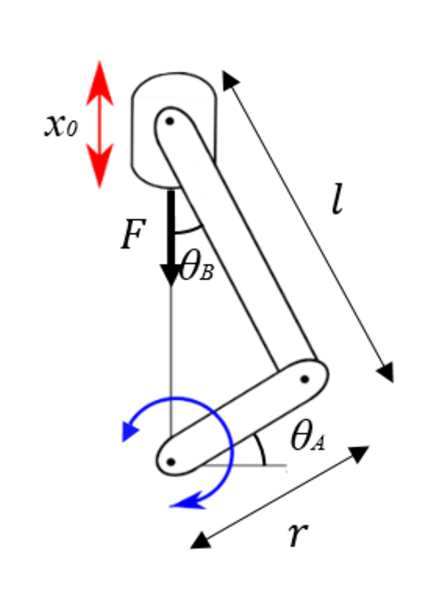
\includegraphics[height=45mm]{figure/slider_crank.eps}
    \vspace*{3mm}
    \caption{Slider Crank Mechanism}
    \label{fig:slider_crank}
  \end{center}
\end{figure}

\vspace{5mm}
\begin{figure}[h]
\begin{center}
    \includegraphics[height=45mm]{figure/mm_pulse.eps}
    \vspace*{3mm}
    \caption{Displacement Pulse}
    \label{fig:mm_to_pulse}
     \end{center}
\end{figure}


\newpage
\subsection{路面部の応答性}
HILS試験機の路面部を作成し応答性を評価した.
HILS試験機の路面部へスイープ入力を与えた結果を示す.
図~\ref{fig:x0sweep_input}~に入力変位を,図~\ref{fig:x0sweep_output}~にレーザ変位計を用いて計測した出力変位の結果を示す.
このとき入力は0.5~Hz~から~10~Hz~の周波数で加速度振幅一定のスイープ状の入力を作成している.ここからはシリアル通信によりモータの位置制御を行っている.

\vspace*{12mm}
\begin{figure}[h]
  \begin{center}
    \includegraphics[height=45mm]{figure/x0sweep_input.eps}
    \vspace*{3mm}
    \caption{Input}
    \label{fig:x0sweep_input}
  \end{center}
\end{figure}

\vspace*{12mm}
 \begin{figure}[h]
  \begin{center}
    \includegraphics[height=45mm]{figure/x0sweep_output.eps}
    \vspace*{3mm}
    \caption{Output}
    \label{fig:x0sweep_output}
  \end{center}
\end{figure}

\newpage
次に,入力変位に対する出力変位の伝達関数を同定し,高速フーリエ変換(FFT)による周波数応答の結果を図~\ref{fig:x0sweep}~に示す.
この結果から,路面部が指令値に対して十分に応答していることを確認した.

% % % ーーーーーーーーーーーーーーーーーーーーーーーーーーーーーーー
% % % Bode diagram
% % %  ーーーーーーーーーーーーーーーーーーーーーーーーーーーーーーー
\vspace{10mm}
\begin{figure}[h]
  \begin{center}
   \includegraphics[height=75mm]{figure/x0sweep.eps}
  \vspace{2mm}
\caption{Bode diagram (Road input)}
\  (Input: Input Displacement, Output: Measurement of Laser Sensor)
  \label{fig:x0sweep}
  \end{center}
\end{figure}
% ーーーーーーーーーーーーーーーーーーーーーーーーーーーーーーーー


\newpage
\subsection{フィードバック要素の計測}
本研究では,HILSシステムのフィードバック要素としてダンパ力を用いている.
ここで,HILS試験機においてロードセルを用いてダンパ力を計測した.振幅~7~mm~振動数~2~Hz~の正弦波状の路面変位を与えた場合の速度に対するダンパ力の図を示す.
図~\ref{fig:liner}~に線形ダンパで計算した結果を,図~\ref{fig:non}~に実際のダンパ力の計測結果を示す.
線形でモデル化したダンパ力の傾きは一定であるのに対し,計測したダンパ力は非線形な力を生じている.
このように,ダンパは複雑な特性を有するため,本システムのフィードバック要素として用いることにした.

% % ーーーーーーーーーーーーーーーーーーーーーーーーーーーーーーー
% % Liner
% %  ーーーーーーーーーーーーーーーーーーーーーーーーーーーーーーー
\vspace{15mm}
\begin{figure}[h]
    \begin{tabular}{cc}
      \begin{minipage}{0.45\hsize}
	\centering
% 	\vspace{20mm}
	  \includegraphics[height=40mm]{figure/damp_sys_liner_time.eps}
	  \begin{center}
	  \vspace{2mm}
	  \ (A) Time Series\
	  \end{center}
	\end{minipage}
       \begin{minipage}{0.5\hsize}
	\centering
% 	\vspace{20mm}
	  \includegraphics[height=40mm]{figure/damp_sys_liner.eps}
	  \begin{center}
	  \vspace{2mm}
	  \ (B) Lissajous Diagram\
	  \end{center}
      \end{minipage}
    \end{tabular}
    \vspace{2mm}
    \caption{Liner Damper}
    \label{fig:liner}
\end{figure}
% % ーーーーーーーーーーーーーーーーーーーーーーーーーーーーーーー
% % Non-liner
% %  ーーーーーーーーーーーーーーーーーーーーーーーーーーーーーーー
\vspace{15mm}
\begin{figure}[h]
    \begin{tabular}{cc}
      \begin{minipage}{0.45\hsize}
	\centering
% 	\vspace{20mm}
	  \includegraphics[height=40mm]{figure/damp_sys_time.eps}
	  \begin{center}
	  \vspace{2mm}
	  \ (A) Time Series\
	  \end{center}
	\end{minipage}
       \begin{minipage}{0.5\hsize}
	\centering
% 	\vspace{20mm}
	  \includegraphics[height=40mm]{figure/damp_sys.eps}
	  \begin{center}
	  \vspace{2mm}
	  \ (B) Lissajous Diagram\
	  \end{center}
      \end{minipage}
    \end{tabular}
    \vspace{2mm}
    \caption{Non-liner Damper}
    \label{fig:non}
\end{figure}


\newpage
\subsection{ハードウェアモデルの同定}
ここでは,開発したHILS試験機を用いてモデルのパラメータを同定する.ハードウェアのモデルでは,線形のパラメータを用いてダンパをモデル化した.
1自由度のHILS試験機にスイープ入力を与え,サスペンションストロークをレーザ変位計を用いて計測した.
図~\ref{fig:1dof_input}~に入力変位を,図~\ref{fig:1dof_output}~にレーザ変位計を用いて計測した出力変位の結果を示す.
このとき入力は0.5~Hz~から~10~Hz~の周波数で振幅一定となるスイープ状の入力を作成している.

\vspace*{12mm}
\begin{figure}[h]
  \begin{center}
    \includegraphics[height=45mm]{figure/1dof_input.eps}
    \vspace*{3mm}
    \caption{Input}
    \label{fig:1dof_input}
  \end{center}
\end{figure}

\vspace*{12mm}
 \begin{figure}[h]
  \begin{center}
    \includegraphics[height=45mm]{figure/1dof_output.eps}
    \vspace*{3mm}
    \caption{Output}
    \label{fig:1dof_output}
  \end{center}
\end{figure}

\newpage
次に,入力変位に対する出力変位の伝達関数を同定し,高速フーリエ変換(FFT)による周波数応答の結果を図~\ref{fig:1dof_sweep}~に示す.
この結果から,路面入力に対する1自由度のHILS試験機のサスペンションストロークの周波数応答を確認した.
この結果から,ハードウェアのモデルを同定し,$c_2$の減衰係数を~7~Ns/m~と決定した.
このパラメータ同定したハードウェアのモデルの路面入力に対するサスペンションストロークの周波数応答を図~\ref{fig:sistem_sweep}~に示す.
ハードウェアの周波数応答特性から~7~Hz~付近で共振が見られ,ゲインが10倍近くなることがわかる.
% % % ーーーーーーーーーーーーーーーーーーーーーーーーーーーーーーー
% % % Bode diagram
% % %  ーーーーーーーーーーーーーーーーーーーーーーーーーーーーーーー
\vspace{10mm}
\begin{figure}[h]
  \begin{center}
   \includegraphics[height=70mm]{figure/1dof_sweep.eps}
  \vspace{2mm}
\caption{Bode Diagram (Testing Machine)}
\  (Input: Input Displacement, Output: Measurement of Laser Sensor)
  \label{fig:1dof_sweep}
  \end{center}
\end{figure}
% ーーーーーーーーーーーーーーーーーーーーーーーーーーーーーーーー
% % % ーーーーーーーーーーーーーーーーーーーーーーーーーーーーーーー
% % % Bode diagram
% % %  ーーーーーーーーーーーーーーーーーーーーーーーーーーーーーーー
\vspace{10mm}
\begin{figure}[h]
  \begin{center}
   \includegraphics[height=70mm]{figure/sistem_doutei.eps}
  \vspace{2mm}
\caption{Bode Diagram (Hardware Model)}
\  (Input: $\bar{x}_0$, Output: $-\bar{x}_1$)
  \label{fig:sistem_sweep}
  \end{center}
\end{figure}
% ーーーーーーーーーーーーーーーーーーーーーーーーーーーーーーーー
\newpage
同定したハードウェアのモデルを図~\ref{fig:serial_send}~のようにしてSimulinkで実現した.
解析モデルの計算結果であるサスペンションストローク~$-{\bar{x}}_1$~から,式(\ref{eq:1DOF_2})を用いて路面変位~$\bar{x}_0$~を計算している.
このとき,路面変位の平滑化を行うために伝達関数を用いた微分手法を用いた.その伝達関数を式(\ref{eq:s})に示す.
式中における時定数~$T$~の値を任意に設定することで平滑化を行うことができる.
しかし,時定数の値を大きく設定するほど微分した値の遅れが大きくなるため,時定数と遅れはトレードオフの関係となる.
今回は周波数~50~Hz~以上の振動を低減するために,時定数は~0.02~を用いた.
また,今回は簡易的に線形ダンパを用いて計算を行った.


\vspace*{-10mm}
\begin{flalign}
\label{eq:1DOF_2}
\ & m_1\ddot{\bar{x}}_1+c_2\dot{\bar{x}}_1+k_1(\bar{x}_1-\bar{x}_0)+k_2\bar{x}_1=0
\end{flalign}

\vspace*{-10mm}
\begin{flalign}
\label{eq:s}
\ & \frac{s}{Ts+1}
\end{flalign}

\vspace{15mm}
\begin{figure}[htp]
  \begin{center}
    \includegraphics[height=100mm]{figure/inverse.eps}
    \vspace{3mm}
    \caption{Hardware Inverse}
    \label{fig:inverse}
  \end{center}
\end{figure}

\newpage
\section{HILSシステムの構築}
\subsection{シミュレーションによる検証}
HILSシステムを構築する前にハードウェアを1自由度のモデルに置き換えたシミュレーションを行った.
このときのブロック線図を図~\ref{fig:block_HILS_sim}~に示す.
図~\ref{fig:sim}~に路面入力に対するサスペンションストロークの結果を示す.解析モデルで計算したサスペンションストロークとハードウェアのモデルで計算した結果を比較している.

% % ーーーーーーーーーーーーーーーーーーーーーーーーーーーーーーー
% % Block diagram
% %  ーーーーーーーーーーーーーーーーーーーーーーーーーーーーーーー
 \vspace{8mm}
\begin{figure}[h]
  \centering
  \includegraphics[height=45mm]{figure/block_HILS_sim.eps}
  \vspace{2mm}
   \caption{Block Diagram}
  \label{fig:block_HILS_sim}
\end{figure}
% ーーーーーーーーーーーーーーーーーーーーーーーーーーーーーーーー

% % ーーーーーーーーーーーーーーーーーーーーーーーーーーーーーーー
% % Step
% %  ーーーーーーーーーーーーーーーーーーーーーーーーーーーーーーー
\vspace{15mm}
\begin{figure}[h]
    \begin{tabular}{cc}
      \begin{minipage}{0.45\hsize}
	\centering
% 	\vspace{20mm}
	  \includegraphics[height=40mm]{figure/input_sine_2_7.eps}
	  \begin{center}
	  \vspace{2mm}
	  \ (A) Road Input (Sine~2~Hz~7~mm)\
	  \end{center}
	\end{minipage}
       \begin{minipage}{0.5\hsize}
	\centering
% 	\vspace{20mm}
	  \includegraphics[height=40mm]{figure/sim_2_7.eps}
	  \begin{center}
	  \vspace{2mm}
	  \ (B) Suspension Stroke\
	  \end{center}
      \end{minipage}
    \end{tabular}
    \vspace{2mm}
    \caption{Simulation Result}
    \label{fig:sim}
\end{figure}

\newpage
\subsection{HILSシステムの評価}
路面部に図~\ref{fig:sine2}~と図~\ref{fig:sine5}~に示す正弦波状の入力を与えた際の,サスペンションストロークをレーザ変位計により計測した.
また,ロードセルを用いて計測したダンパ力を用いてHILSシステムを構築した結果を示す.
このとき,力計測には50Hzのローパスフィルタによる処理を行い,変位計測では100Hzのローパスフィルタによる処理を行っている.そのため,入力にも同様の処理を行い結果を比較した.
\vspace{15mm}
% \vspace{1mm}
\begin{figure}[h]
  \centering
   \includegraphics[height=45mm]{figure/input_sine_2_7.eps}
  \vspace{2mm}
\caption{Road Input (Sine~2~Hz~7~mm)}
  \label{fig:sine2}
\end{figure}

\vspace{15mm}
% \vspace{1mm}
\begin{figure}[h]
  \centering
   \includegraphics[height=45mm]{figure/input_sine_5_2.eps}
  \vspace{2mm}
\caption{Road Input (Sine~5~Hz~2~mm)}
  \label{fig:sine5}
\end{figure}

\newpage
解析モデルで計算したサスペンションストロークと,レーザ変位計を用いて計測したサスペンションストロークの比較結果と計測したダンパ力を示す.
図~\ref{fig:sine_2}~に振幅~7~mm~振動数~2~Hz~の,図~\ref{fig:sine_5}~には振幅~2~mm~振動数~5~Hz~の正弦波入力を与えた結果を示す.
それぞれ(A)にサスペンションストロークの解析モデルでの計算結果とレーザ変位計の計測結果を比較したものを,(B)にロードセルを用いて計測しフィードバック要素として用いているダンパ力を示す.
\par
(A)のグラフで見られるサスペンションストロークの計算結果と計測結果の違いはモデル化誤差による影響である.振
動数~2~Hz~では解析モデルの計算結果にレーザ変位計の計測結果がよく対応している結果が得られた.
振動数が高くなるにつれて解析モデルの計算結果とハードウェアの挙動が乖離する結果となった.
これは,ハードウェアの逆モデルで線形パラメータを用いたことによるダンパの速度に対する非線形性の影響が考えられる.
% % ーーーーーーーーーーーーーーーーーーーーーーーーーーーーーーー
% % Step
% %  ーーーーーーーーーーーーーーーーーーーーーーーーーーーーーーー
\vspace{10mm}
\begin{figure}[h]
    \begin{tabular}{cc}
      \begin{minipage}{0.45\hsize}
	\centering
	  \includegraphics[height=40mm]{figure/hils_sine_2_7.eps}
	  \begin{center}
	  \vspace{2mm}
	  \ (A) Suspension Stroke\
	  \end{center}
	\end{minipage}
       \begin{minipage}{0.45\hsize}
	\centering
	  \includegraphics[height=40mm]{figure/hils_sine_2_7_damp.eps}
	  \begin{center}
	  \vspace{2mm}
	  \ (B) Damper Force\
	  \end{center}
      \end{minipage}
    \end{tabular}
    \vspace{2mm}
    \caption{Road Input (Sine 2~Hz~7~mm)}
    \label{fig:sine_2}
\end{figure}

% % ーーーーーーーーーーーーーーーーーーーーーーーーーーーーーーー
% % Step
% %  ーーーーーーーーーーーーーーーーーーーーーーーーーーーーーーー
\vspace{10mm}
\begin{figure}[h]
    \begin{tabular}{cc}
      \begin{minipage}{0.45\hsize}
	\centering
	  \includegraphics[height=40mm]{figure/hils_sine_5_2.eps}
	  \begin{center}
	  \vspace{2mm}
	  \ (A) Suspension Stroke\
	  \end{center}
	\end{minipage}
       \begin{minipage}{0.5\hsize}
	\centering
	  \includegraphics[height=40mm]{figure/hils_sine_5_2_damp.eps}
	  \begin{center}
	  \vspace{2mm}
	  \ (B) Damper Force\
	  \end{center}
      \end{minipage}
    \end{tabular}
    \vspace{2mm}
    \caption{Road Input (Sine 5~Hz~2~mm)}
    \label{fig:sine_5}
\end{figure}

\newpage
また,正弦波入力による入力を与えてすぐは波形が安定しないため,安定した5秒後以降の波形をモデル化誤差の影響評価では用いる.
図~\ref{fig:sine2_0}~に振動数~2~Hz~7~mm~の入力を与えた際のサスペンションストロークの結果を,図~\ref{fig:sine5_0}~に振動数~5~Hz~2~mm~の入力を与えた際の結果を示す.

\vspace{15mm}
% \vspace{1mm}
\begin{figure}[h]
  \centering
   \includegraphics[height=45mm]{figure/hils_sine_2_7_0s.eps}
  \vspace{2mm}
\caption{Suspension Stroke (Sine~2~Hz~7~mm)}
  \label{fig:sine2_0}
\end{figure}

\vspace{15mm}
% \vspace{1mm}
\begin{figure}[h]
  \centering
   \includegraphics[height=45mm]{figure/hils_sine_5_2_0s.eps}
  \vspace{2mm}
\caption{Suspension Stroke (Sine~5~Hz~2~mm)}
  \label{fig:sine5_0}
\end{figure}

\newpage
次に,ステップ入力による評価を行った.
図~\ref{fig:step2}~に示す~2~mm~のステップ入力を与えた際の,サスペンションストロークを図~\ref{fig:step_2}~に示す.
それぞれ解析モデルの計算結果とレーザ変位計による計測結果を比較している.
このとき,瞬間的な入力を行ったことにより入力に対して高い振動数での共振が見られた.これは,7~Hz~付近で装置の共振点の影響が出たためだと考えられる.
図~\ref{fig:1dof_sweep}~に示すボード線図で共振点について確認することができる.
また,ばね上で用いたばねの質量により振動し,ばねが波打つような現象が見られた.これも,共振点付近の現象に影響していると考えられる.

\vspace{10mm}
\begin{figure}[h]
  \begin{center}
   \includegraphics[height=40mm]{figure/step_2.eps}
  \vspace{2mm}
  \caption{Road Input (Step 2mm)}
  \end{center}
  \label{fig:step2}
\end{figure}

% ーーーーーーーーーーーーーーーーーーーーーーーーーーーーーーー
% Step
%  ーーーーーーーーーーーーーーーーーーーーーーーーーーーーーーー
\vspace{10mm}
\begin{figure}[h]
    \begin{tabular}{cc}
      \begin{minipage}{0.45\hsize}
	\begin{center}
	  \includegraphics[height=40mm]{figure/hils_step_2.eps}
	  \end{center}
	  \begin{center}
	  \vspace{2mm}
	  \ (A) Suspension Stroke
	  \end{center}
	\end{minipage}
       \begin{minipage}{0.5\hsize}
	\begin{center}
	  \includegraphics[height=40mm]{figure/hils_step_2_damp.eps}
	  \end{center}
	  \begin{center}
	  \vspace{2mm}
	  \ (B) Damper Force
	  \end{center}
	   \end{minipage}
           \end{tabular}
	\label{fig:step_2}
      \begin{center}
      \vspace{2mm}
      \caption{Road Input (Step 2mm)}
    \end{center}
\end{figure}

\newpage
図~\ref{fig:step46}~に示す~4~mm~と~6~mm~のステップ入力を与えた際の,サスペンションストロークを図~\ref{fig:step_4}~と図~\ref{fig:step_6}~に示す.

% ーーーーーーーーーーーーーーーーーーーーーーーーーーーーーーー
% Step46
%  ーーーーーーーーーーーーーーーーーーーーーーーーーーーーーーー
\vspace{10mm}
\begin{figure}[h]
    \begin{tabular}{cc}
      \begin{minipage}{0.45\hsize}
	\begin{center}
	  \includegraphics[height=35mm]{figure/step_4.eps}
	  \end{center}
	  \begin{center}
	  \vspace{-2mm}
	  \ (A) Step 4mm
	  \end{center}
	\end{minipage}
       \begin{minipage}{0.5\hsize}
	\begin{center}
	  \includegraphics[height=35mm]{figure/step_4.eps}
	  \end{center}
	  \begin{center}
	  \vspace{-2mm}
	  \ (B) Step 6mm
	  \end{center}
	   \end{minipage}
           \end{tabular}
	\label{fig:step46}
      \begin{center}
      \vspace{-2mm}
      \caption{Road Input}
    \end{center}
\end{figure}
% ーーーーーーーーーーーーーーーーーーーーーーーーーーーーーーー
% Step
%  ーーーーーーーーーーーーーーーーーーーーーーーーーーーーーーー
% \vspace{2mm}
\begin{figure}[h]
    \begin{tabular}{cc}
      \begin{minipage}{0.45\hsize}
	\begin{center}
	  \includegraphics[height=35mm]{figure/hils_step_4.eps}
	  \end{center}
	  \begin{center}
	  \vspace{-2mm}
	  \ (A) Suspension Stroke
	  \end{center}
	\end{minipage}
       \begin{minipage}{0.5\hsize}
	\begin{center}
	  \includegraphics[height=35mm]{figure/hils_step_4_damp.eps}
	  \end{center}
	  \begin{center}
	  \vspace{-2mm}
	  \ (B) Damper Force
	  \end{center}
	   \end{minipage}
           \end{tabular}
	\label{fig:step_4}
      \begin{center}
      \vspace{-2mm}
      \caption{Road Input (Step 4mm)}
    \end{center}
\end{figure}

% ーーーーーーーーーーーーーーーーーーーーーーーーーーーーーーー
% Step
%  ーーーーーーーーーーーーーーーーーーーーーーーーーーーーーーー
% \vspace{2mm}
\begin{figure}[h]
    \begin{tabular}{cc}
      \begin{minipage}{0.45\hsize}
	\begin{center}
	  \includegraphics[height=35mm]{figure/hils_step_6.eps}
	  \end{center}
	  \begin{center}
	  \vspace{-2mm}
	  \ (A) Suspension Stroke
	  \end{center}
	\end{minipage}
       \begin{minipage}{0.5\hsize}
	\begin{center}
	  \includegraphics[height=35mm]{figure/hils_step_6_damp.eps}
	  \end{center}
	  \begin{center}
	  \vspace{-2mm}
	  \ (B) Damper Force
	  \end{center}
	   \end{minipage}
           \end{tabular}
	\label{fig:step_6}
      \begin{center}
      \vspace{2mm}
      \caption{Road Input (Step 6mm)}
    \end{center}
\end{figure}


\newpage
\section{モデル化誤差の影響評価}
\subsection{ばね定数}
\subsubsection{シミュレーション結果}
まずモデル化誤差の影響をシミュレーションにより検証した.図~\ref{fig:sim_k2}~の(A)に示す路面入力を与え,解析モデルのばね定数$k_2$を変更した場合の結果を図~\ref{fig:sim_k2}~の(B)と図~\ref{fig:sim_k2_1}~示す.
この結果では,モデル化誤差による影響は見られなかった.
シミュレーションではダンパ力は線形としているため,影響は見られなかったと考えられる.

% % ーーーーーーーーーーーーーーーーーーーーーーーーーーーーーーー
% % Step
% %  ーーーーーーーーーーーーーーーーーーーーーーーーーーーーーーー
\vspace{15mm}
\begin{figure}[h]
    \begin{tabular}{cc}
      \begin{minipage}{0.45\hsize}
	\centering
% 	\vspace{20mm}
	  \includegraphics[height=40mm]{figure/input_sine_2_5.eps}
	  \begin{center}
	  \vspace{2mm}
	  \ (A) Road Input (Sine~2~Hz~5~mm)\
	  \end{center}
	\end{minipage}
       \begin{minipage}{0.5\hsize}
	\centering
% 	\vspace{20mm}
	  \includegraphics[height=40mm]{figure/sim_2_5_k2_405.eps}
	  \begin{center}
	  \vspace{2mm}
	  \ (B) Suspension Stroke\
	  \end{center}
      \end{minipage}
    \end{tabular}
    \vspace{2mm}
    \caption{$k_2$ = 405~[N/m]}
    \label{fig:sim_k2}
\end{figure}

% % ーーーーーーーーーーーーーーーーーーーーーーーーーーーーーーー
% % Step
% %  ーーーーーーーーーーーーーーーーーーーーーーーーーーーーーーー
\vspace{15mm}
\begin{figure}[h]
    \begin{tabular}{cc}
      \begin{minipage}{0.45\hsize}
	\centering
% 	\vspace{20mm}
	  \includegraphics[height=40mm]{figure/sim_2_5_k2_300.eps}
	  \begin{center}
	  \vspace{2mm}
	  \ (A) $k_2$ = 300~[N/m]\
	  \end{center}
	\end{minipage}
       \begin{minipage}{0.5\hsize}
	\centering
% 	\vspace{20mm}
	  \includegraphics[height=40mm]{figure/sim_2_5_k2_500.eps}
	  \begin{center}
	  \vspace{2mm}
	  \ (B) $k_2$ = 500~[N/m]\
	  \end{center}
      \end{minipage}
    \end{tabular}
    \vspace{2mm}
    \caption{Suspension Stroke}
    \label{fig:sim_k2_1}
\end{figure}

\newpage
次に,図~\ref{fig:sim_k1}~の(A)に示す路面入力を与え,解析モデルのばね定数$k_1$を変更した場合の結果を図~\ref{fig:sim_k1}~の(B)と図~\ref{fig:sim_k1_1}~に示す.
この結果から,ばね定数が小さくなるほど振幅が大きく離れる傾向が見られた.

% % ーーーーーーーーーーーーーーーーーーーーーーーーーーーーーーー
% % Spring
% %  ーーーーーーーーーーーーーーーーーーーーーーーーーーーーーーー
\vspace{15mm}
\begin{figure}[h]
    \begin{tabular}{c}
      \begin{minipage}{0.45\hsize}
	\begin{center}
% 	\vspace{20mm}
	  \includegraphics[height=40mm]{figure/input_sine_5_2.eps}
	\end{center}
	\begin{center}
	  \vspace{2mm}
	  \ (A) Road Input (Sine~5~Hz~2~mm) \
	  \end{center}
      \end{minipage}
      \begin{minipage}{0.5\hsize}
	\begin{center}
% 	\vspace{20mm}
	  \includegraphics[height=40mm]{figure/sim_5_2_k1_2200.eps}
	\end{center}
	\begin{center}
	  \vspace{2mm}
	  \ (B) Suspension Stroke \
	  \end{center}
      \end{minipage}
    \end{tabular}
    \vspace{2mm}
    \caption{$k_1$ = 2200~[N/m]}
    \label{fig:sim_k1}
\end{figure}
% % ーーーーーーーーーーーーーーーーーーーーーーーーーーーーーーー
% % Spring
% %  ーーーーーーーーーーーーーーーーーーーーーーーーーーーーーーー
\vspace{15mm}
\begin{figure}[h]
    \begin{tabular}{c}
      \begin{minipage}{0.45\hsize}
	\begin{center}
% 	\vspace{20mm}
	  \includegraphics[height=40mm]{figure/sim_5_2_k1_1000.eps}
	\end{center}
	\begin{center}
	  \vspace{2mm}
	  \ (A) $k_1$ = 1000~[N/m]\
	  \end{center}
      \end{minipage}
      \begin{minipage}{0.5\hsize}
	\begin{center}
% 	\vspace{20mm}
	  \includegraphics[height=40mm]{figure/sim_5_2_k1_500.eps}
	\end{center}
	\begin{center}
	  \vspace{2mm}
	  \ (B) $k_1$ = 500~[N/m]\
	  \end{center}
      \end{minipage}
    \end{tabular}
    \vspace{2mm}
    \caption{Suspension Stroke}
    \label{fig:sim_k1_1}
\end{figure}

\newpage
次に,図~\ref{fig:sim_k1_s}~の(A)に示す路面入力を与え,解析モデルのばね定数$k_1$を変更した場合の結果を図~\ref{fig:sim_k1_s}~の(B)と図~\ref{fig:sim_k1_s1}~に示す.
この結果から,ばね定数が小さくなるほど振幅が大きく離れる傾向が見られた.
また,1自由度モデルのサスペンションストロークの結果に振動が見られた.
% % ーーーーーーーーーーーーーーーーーーーーーーーーーーーーーーー
% % Spring
% %  ーーーーーーーーーーーーーーーーーーーーーーーーーーーーーーー
\vspace{15mm}
\begin{figure}[h]
    \begin{tabular}{c}
      \begin{minipage}{0.45\hsize}
	\begin{center}
% 	\vspace{20mm}
	  \includegraphics[height=40mm]{figure/step_2.eps}
	\end{center}
	\begin{center}
	  \vspace{2mm}
	  \ (A) Input (Step 2mm)\
	  \end{center}
      \end{minipage}
      \begin{minipage}{0.5\hsize}
	\begin{center}
% 	\vspace{20mm}
	  \includegraphics[height=40mm]{figure/sim_2_k1_2200.eps}
	\end{center}
	\begin{center}
	  \vspace{2mm}
	  \ (B) Suspension Stroke\
	  \end{center}
      \end{minipage}
    \end{tabular}
    \vspace{2mm}
    \caption{$k_1$ = 2200~[N/m]}
    \label{fig:sim_k1_s}
\end{figure}

% % ーーーーーーーーーーーーーーーーーーーーーーーーーーーーーーー
% % Spring
% %  ーーーーーーーーーーーーーーーーーーーーーーーーーーーーーーー
\vspace{15mm}
\begin{figure}[h]
    \begin{tabular}{c}
      \begin{minipage}{0.45\hsize}
	\begin{center}
% 	\vspace{20mm}
	  \includegraphics[height=40mm]{figure/sim_2_k1_1000.eps}
	\end{center}
	\begin{center}
	  \vspace{2mm}
	  \ (A) $k_1$ = 1000~[N/m]\
	  \end{center}
      \end{minipage}
      \begin{minipage}{0.5\hsize}
	\begin{center}
% 	\vspace{20mm}
	  \includegraphics[height=40mm]{figure/sim_2_k1_500.eps}
	\end{center}
	\begin{center}
	  \vspace{2mm}
	  \ (B) $k_1$ = 500~[N/m]\
	  \end{center}
      \end{minipage}
    \end{tabular}
    \vspace{2mm}
    \caption{Suspension Stroke}
    \label{fig:sim_k1_s1}
\end{figure}


\newpage
\subsubsection{HILS試験}
次に,開発したHILSシステムを用いてモデル化誤差の影響を評価した.
解析モデルに意図的にモデル化誤差を与え,サスペンションストロークの解析モデルと計測結果を比較した.
図~\ref{fig:2_5}~の振幅~5~mm~振動数~2~Hz~の正弦波入力を行った場合のサスペンションストロークをばね定数$k_2$を変更した場合を比較する.
図~\ref{fig:k2_405}~に解析モデルのばね定数$k_2$を~405~N/m~の結果を示す.
% \noindent


\vspace{15mm}
% \vspace{1mm}
\begin{figure}[h]
  \centering
   \includegraphics[height=45mm]{figure/input_sine_2_5.eps}
  \vspace{2mm}
\caption{Road Input (Sine~2~Hz~5~mm)}
  \label{fig:2_5}
\end{figure}

% % ーーーーーーーーーーーーーーーーーーーーーーーーーーーーーーー
% % Step
% %  ーーーーーーーーーーーーーーーーーーーーーーーーーーーーーーー
\vspace{15mm}
\begin{figure}[h]
    \begin{tabular}{cc}
      \begin{minipage}{0.45\hsize}
	\centering
	  \includegraphics[height=40mm]{figure/2_5_405.eps}
	  \begin{center}
	  \vspace{2mm}
	  \ (A) Suspension Stroke\
	  \end{center}
	\end{minipage}
       \begin{minipage}{0.5\hsize}
	\centering
	  \includegraphics[height=40mm]{figure/2_5_405_damp.eps}
	  \begin{center}
	  \vspace{2mm}
	  \ (B) Damper Force\
	  \end{center}
      \end{minipage}
    \end{tabular}
    \vspace{2mm}
    \caption{$k_2$ = 405~[N/m]}
    \label{fig:k2_405}
\end{figure}

\newpage
次に,モデル化誤差を与えた結果を示す.
図~\ref{fig:k2_300}~にばね定数$k_2$が~300~N/m~の結果を,図~\ref{fig:k2_500}~にばね定数$k_2$が~500~N/m~の結果を示す.
この結果から,ばね定数が小さくなると解析モデルの計算結果に比べて計測結果の振幅が小さくなり,ばね定数が大きくなると解析モデルの計算結果に比べて振幅が大きくなる傾向が見られた.
このことから,モデル化誤差により解析モデルとハードウェアの挙動に差異が生じたことがわかる.
% % ーーーーーーーーーーーーーーーーーーーーーーーーーーーーーーー
% % Step
% %  ーーーーーーーーーーーーーーーーーーーーーーーーーーーーーーー
\vspace{10mm}
\begin{figure}[h]
    \begin{tabular}{cc}
      \begin{minipage}{0.45\hsize}
	\centering
	\vspace{20mm}
	  \includegraphics[height=40mm]{figure/2_5_300.eps}
	  \begin{center}
	  \vspace{2mm}
	  \ (A) Suspension Stroke\
	  \end{center}
	\end{minipage}
       \begin{minipage}{0.5\hsize}
	\centering
	\vspace{20mm}
	  \includegraphics[height=40mm]{figure/2_5_300_damp.eps}
	  \begin{center}
	  \vspace{2mm}
	  \ (B) Damper Force\
	  \end{center}
      \end{minipage}
    \end{tabular}
    \vspace{2mm}
    \caption{$k_2$ = 300~[N/m]}
    \label{fig:k2_300}
\end{figure}

% % ーーーーーーーーーーーーーーーーーーーーーーーーーーーーーーー
% % Step
% %  ーーーーーーーーーーーーーーーーーーーーーーーーーーーーーーー
\vspace{10mm}
\begin{figure}[h]
    \begin{tabular}{cc}
      \begin{minipage}{0.45\hsize}
	\centering
	  \includegraphics[height=40mm]{figure/2_5_500.eps}
	  \begin{center}
	  \vspace{2mm}
	  \ (A) Suspension Stroke\
	  \end{center}
	\end{minipage}
       \begin{minipage}{0.5\hsize}
	\centering
	  \includegraphics[height=40mm]{figure/2_5_500_damp.eps}
	  \begin{center}
	  \vspace{2mm}
	  \ (B) Damper Force\
	  \end{center}
      \end{minipage}
    \end{tabular}
    \vspace{2mm}
    \caption{$k_2$ = 500~[N/m]}
    \label{fig:k2_500}
\end{figure}

\newpage
次に解析モデルのタイヤの縦ばね剛性$k_1$を変更し,図~\ref{fig:5_2_}~に示す~5Hz~2mm~の正弦波入力によるサスペンションストロークの結果を比較する.
図~\ref{fig:5_2_2200}~に$k_1$が~2200~N/m~の結果を,図~\ref{fig:5_2_1000}~に$k_1$が~1000~N/m~の結果を示す.
ばね定数が変化したことより,振幅が大きく変化したことがわかる.これはばね下共振付近の現象を見ているため,ばね定数の変化が大きく現れたと言える.

\vspace{2mm}
% \vspace{1mm}
\begin{figure}[h]
  \centering
   \includegraphics[height=45mm]{figure/input_sine_5_2.eps}
  \vspace{2mm}
\caption{Road Input (Sine~5~Hz~2~mm)}
  \label{fig:5_2_}
\end{figure}

% % ーーーーーーーーーーーーーーーーーーーーーーーーーーーーーーー
% % Spring
% %  ーーーーーーーーーーーーーーーーーーーーーーーーーーーーーーー
\vspace{10mm}
\begin{figure}[h]
    \begin{tabular}{c}
      \begin{minipage}{0.45\hsize}
	\begin{center}
	  \includegraphics[height=40mm]{figure/hils_sine_5_2.eps}
	\end{center}
	\begin{center}
	  \vspace{2mm}
	  \ (A) Suspension Stroke \
	  \end{center}
      \end{minipage}
      \begin{minipage}{0.5\hsize}
	\begin{center}
	  \includegraphics[height=40mm]{figure/hils_sine_5_2_damp.eps}
	\end{center}
	\begin{center}
	  \vspace{2mm}
	  \ (B) Damper Force \
	  \end{center}
      \end{minipage}
    \end{tabular}
    \vspace{2mm}
    \caption{$k_1$ = 2200~[N/m]}
    \label{fig:5_2_2200}
\end{figure}
% % ーーーーーーーーーーーーーーーーーーーーーーーーーーーーーーー
% % Spring
% %  ーーーーーーーーーーーーーーーーーーーーーーーーーーーーーーー
\vspace{10mm}
\begin{figure}[h]
    \begin{tabular}{c}
      \begin{minipage}{0.45\hsize}
	\begin{center}
	  \includegraphics[height=40mm]{figure/hils_sine_5_2_1000.eps}
	\end{center}
	\begin{center}
	  \vspace{2mm}
	  \ (A) Suspension Stroke\
	  \end{center}
      \end{minipage}
      \begin{minipage}{0.5\hsize}
	\begin{center}
	  \includegraphics[height=40mm]{figure/hils_sine_5_2_1000_damp.eps}
	\end{center}
	\begin{center}
	  \vspace{2mm}
	  \ (B) Damper Force\
	  \end{center}
      \end{minipage}
    \end{tabular}
    \vspace{2mm}
    \caption{$k_1$ = 1000~[N/m]}
    \label{fig:5_2_1000}
\end{figure}


\newpage
次に解析モデルのタイヤの縦ばね剛性を変更し,図~\ref{fig:step_2_}~に示す~2~mm~のステップ入力によるサスペンションストロークの結果を図~\ref{fig:step_1000}~に示す.
細かい振動が見えているが全体として,振幅が大きくなる傾向は見ることができた.

\vspace{10mm}
\begin{figure}[h]
  \begin{center}
   \includegraphics[height=40mm]{figure/step_2.eps}
  \vspace{2mm}
  \caption{Input (Step 2mm)}
  \end{center}
  \label{fig:step_2_}
\end{figure}

% % ーーーーーーーーーーーーーーーーーーーーーーーーーーーーーーー
% % Spring
% %  ーーーーーーーーーーーーーーーーーーーーーーーーーーーーーーー
\vspace{10mm}
\begin{figure}[h]
    \begin{tabular}{c}
      \begin{minipage}{0.45\hsize}
	\begin{center}
	  \includegraphics[height=40mm]{figure/hils_step.eps}
	\end{center}
	\begin{center}
	  \vspace{2mm}
	  \ (A) $k_1$ = 2200~[N/m]\
	  \end{center}
      \end{minipage}
      \begin{minipage}{0.5\hsize}
	\begin{center}
	  \includegraphics[height=40mm]{figure/hils_step_1000.eps}
	\end{center}
	\begin{center}
	  \vspace{2mm}
	  \ (B) $k_1$ = 1000~[N/m]\
	  \end{center}
      \end{minipage}
    \end{tabular}
    \vspace{2mm}
    \caption{Step (2mm)}
    \label{fig:step_1000}
\end{figure}



\newpage
\subsection{ハードウェアの摩擦}
次に,解析モデルにモデル化誤差としてハードウェアの摩擦を考慮した場合の解析結果を示す.
式~(\ref{eq:friction})~で示す摩擦力を解析モデルのばね上ばね下間に考慮し評価を行った.$F~$は最大摩擦力,$\dot{x}_2$はばね上速度,$\dot{x}_1$はばね下速度である.
\vspace*{-2mm}
\begin{flalign}
\label{eq:friction}
\ & f=Ftanh(\dot{x}_2-\dot{x}_1)
\end{flalign}
\vspace*{-4mm}
\par
図~\ref{fig:force}~のように最大摩擦力を変化させた摩擦力を考慮し,図~\ref{fig:2_7}~に示す振幅~7~mm~振動数~2~Hz~の正弦波入力を与えた場合のサスペンションストロークを比較する.

% % ーーーーーーーーーーーーーーーーーーーーーーーーーーーーーーー
% % force
% %  ーーーーーーーーーーーーーーーーーーーーーーーーーーーーーーー
\vspace{10mm}
\begin{figure}[h]
	\begin{center}
	  \includegraphics[height=40mm]{figure/friction.eps}
	  \end{center}
    \vspace{2mm}
    \caption{Friction Force}
    \label{fig:force}
\end{figure}


\vspace{15mm}
% \vspace{1mm}
\begin{figure}[h]
  \centering
   \includegraphics[height=45mm]{figure/input_sine_2_7.eps}
  \vspace{2mm}
\caption{Road Input (Sine~2~Hz~7~mm)}
  \label{fig:2_7}
\end{figure}


\newpage
\subsubsection{シミュレーション結果}
まず,解析モデルにハードウェアの摩擦を考慮した場合についてシミュレーションにより検証した.摩擦を考慮していない場合の結果を図~\ref{fig:sim_f}~に示す.
図~\ref{fig:sim_f_1}~には最大摩擦力が~2~N~のサスペンションストロークの結果を,図~\ref{fig:tanh2}~には~4~N~の結果を示す.
% % ーーーーーーーーーーーーーーーーーーーーーーーーーーーーーーー
% % Step
% %  ーーーーーーーーーーーーーーーーーーーーーーーーーーーーーーー

\vspace{15mm}
% \vspace{1mm}
\begin{figure}[h]
  \centering
   \includegraphics[height=40mm]{figure/sim_2_7_F_0.eps}
  \vspace{2mm}
\caption{without Friction(F=0)}
  \label{fig:sim_f}
\end{figure}

% % ーーーーーーーーーーーーーーーーーーーーーーーーーーーーーーー
% % Step
% %  ーーーーーーーーーーーーーーーーーーーーーーーーーーーーーーー
\vspace{10mm}
\begin{figure}[h]
    \begin{tabular}{cc}
      \begin{minipage}{0.45\hsize}
	\centering
	\vspace{20mm}
	  \includegraphics[height=40mm]{figure/sim_2_7_F_2.eps}
	  \begin{center}
	  \vspace{2mm}
	  \ (A) with Friction(F=2)\
	  \end{center}
	\end{minipage}
       \begin{minipage}{0.5\hsize}
	\centering
	\vspace{20mm}
	  \includegraphics[height=40mm]{figure/sim_2_7_F_4.eps}
	  \begin{center}
	  \vspace{2mm}
	  \ (B) with Friction(F=4)\
	  \end{center}
      \end{minipage}
    \end{tabular}
    \vspace{2mm}
    \caption{Suspension Stroke}
    \label{fig:sim_f_1}
\end{figure}



\newpage
\subsubsection{HILS試験}
図~\ref{fig:tanh0}~に摩擦を考慮していない場合の結果を示す.図~\ref{fig:tanh2}~には最大摩擦力が~2~N~のサスペンションストロークの結果を,図~\ref{fig:tanh2}~には~4~N~の結果を示す.
最大~2~N~の摩擦を付与した場合は,解析モデルの計算結果とレーザ変位計の計測結果が近づいた.しかし,最大~4~N~の摩擦を付与した場合には振幅に変化が見られ,システム自体の挙動が変化したことがわかる.
このことからモデル化誤差の影響により,システム自体の挙動が変化し,解析モデルの計算結果とハードウェアの挙動の関係にも変化が生じることがわかる.
% % ーーーーーーーーーーーーーーーーーーーーーーーーーーーーーーー
% % Step
% %  ーーーーーーーーーーーーーーーーーーーーーーーーーーーーーーー
\vspace{2mm}
\begin{figure}[h]
    \begin{tabular}{cc}
      \begin{minipage}{0.45\hsize}
	\centering
	  \includegraphics[height=40mm]{figure/hils_sine_2_7.eps}
	  \begin{center}
	  \vspace{2mm}
	  \ (A) Suspension Stroke\
	  \end{center}
	\end{minipage}
       \begin{minipage}{0.5\hsize}
	\centering
	  \includegraphics[height=40mm]{figure/hils_sine_2_7_damp.eps}
	  \begin{center}
	  \vspace{2mm}
	  \ (B) Damper Force\
	  \end{center}
      \end{minipage}
    \end{tabular}
    \vspace{2mm}
    \caption{without Friction(F=0)}
    \label{fig:tanh0}
\end{figure}

% % ーーーーーーーーーーーーーーーーーーーーーーーーーーーーーーー
% % Step
% %  ーーーーーーーーーーーーーーーーーーーーーーーーーーーーーーー
\vspace{2mm}
\begin{figure}[h]
    \begin{tabular}{cc}
      \begin{minipage}{0.45\hsize}
	\centering
	  \includegraphics[height=40mm]{figure/2_7_tanh2.eps}
	  \begin{center}
	  \vspace{2mm}
	  \ (A) Suspension Stroke\
	  \end{center}
	\end{minipage}
       \begin{minipage}{0.5\hsize}
	\centering
	  \includegraphics[height=40mm]{figure/2_7_tanh2_damp.eps}
	  \begin{center}
	  \vspace{2mm}
	  \ (B) Damper Force\
	  \end{center}
      \end{minipage}
    \end{tabular}
    \vspace{2mm}
    \caption{with Friction(F=2)}
    \label{fig:tanh2}
\end{figure}

% % ーーーーーーーーーーーーーーーーーーーーーーーーーーーーーーー
% % Step
% %  ーーーーーーーーーーーーーーーーーーーーーーーーーーーーーーー
\vspace{2mm}
\begin{figure}[h]
    \begin{tabular}{cc}
      \begin{minipage}{0.45\hsize}
	\centering
	  \includegraphics[height=40mm]{figure/2_7_tanh4.eps}
	  \begin{center}
	  \vspace{2mm}
	  \ (A) Suspension Stroke\
	  \end{center}
	\end{minipage}
       \begin{minipage}{0.5\hsize}
	\centering
	  \includegraphics[height=40mm]{figure/2_7_tanh4_damp.eps}
	  \begin{center}
	  \vspace{2mm}
	  \ (B) Damper Force\
	  \end{center}
      \end{minipage}
    \end{tabular}
    \vspace{2mm}
    \caption{with Friction(F=4)}
    \label{fig:tanh4}
\end{figure}


\newpage
\section{結論}
HILSシステムは解析モデルの計算結果に基づいてハードウェアへの入力を決定し,システム全体の挙動を再現する.そのため,解析モデルの精度はHILSシステムの再現性に影響を及ぼす.
そこで本研究では,HILSシステムにおけるモデル化誤差の影響を評価することを目的として,自動車のタイヤ-サスペンション系の上下挙動を模擬したHILS試験機を新たに開発しモデル化誤差がHILSシステムに及ぼす影響を評価した.

HILSシステムのソフトウェア部とハードウェア部の構成を検討した.ソフトウェア部でアクチュエータの制御と計測環境を構築した.また,ハードウェア部としてHILS試験機を開発し,アクチュエータとしてサーボモータを用いた.
アクチュエータの特性を評価するためにスイープ状の入力を与え周波数応答について確認した.本試験の評価範囲においてアクチュエータが十分に応答できることを確認した.
また,HILS試験機を開発するにあたり,諸元の検討やダンパ,ばねの選定などを行った.
そして,HILS試験機で計測したダンパ力をフィードバックしサスペンションストロークを実現するHILSシステムを開発した.
ハードウェアをモデルに置き換えHILSシステムのシミュレーションによる検証を行った.また,解析モデルを変更した際のHILSシステムへの影響をシミュレーションで確認した.
そして,HILS試験機を用いてHILSシステムを構築し,モデル化誤差の影響を評価した.解析モデルにモデル化誤差を与え,サスペンションストロークの結果を比較した.
このことから,HILSシステムにおいてモデル化誤差がシステムの解析結果に影響を及ぼすことを確認した.

開発した試験機を用いてHILSシステムを構築し,解析モデルの計算結果とハードウェアの計測結果を比較することで,上下変位の解析結果を確認した.
また,モデル化誤差を変更してHILSシステムの上下変位を比較することで,モデル化誤差がHILSシステムの再現性に及ぼす影響を評価した.

\newpage
\begin{thebibliography}{99}
\bibitem{uno}宇野 高明, 車両運動性能とシャシーメカニズム, グランプリ出版,1994
\bibitem{nasu}茄子川 捷久,宮下 義孝,汐川 満則,自動車の走行性能と試験法,山海堂,2004
\bibitem{shiiba}椎葉太一,河内亮,森田恵介, リアルタイム車両運動解析を用いたタイヤ-サスペンション特性評価システムの開発, 日本機械学会論文集,C編Vol.76 No.766(2010), pp.1576-1581
\bibitem{bmw}$\rm{http://www.nicole-bmw.co.jp/jp/nicole-bmw/ja/index.html}$
\bibitem{yamaguchi}山口輝也, 実ヨーダンパを用いたHardware-In-the-Loopシミュレーションによる鉄道車両の蛇行動安定性試験(試験環境の構築と安定的な検証), 日本機械学会論文集,C編Vol.79 No.806(2013-10), pp.131-142
\bibitem{yamato}大和宏一朗,車両のダイナミクスを考慮したタイヤ-サスペンションHILSシステムの開発と評価,2007年度 修士学位請求論文(2007)
\bibitem{dspace}$\rm{http://www.dspace.com/ja/jpn/home.cfm}$
\bibitem{2dof}社団法人\ 自動車技術会,自動車技術ハンドブック5設計(シャシ)編,社団法人\ 自動車技術会,(1990),p.25
\bibitem{GitHub}$\rm{https://github.com/ethz-asl/matlab_epos_library}$
\bibitem{maxon}$\rm{http://academy.maxonjapan.co.jp/mmc}$
\end{thebibliography}



\newpage
\section*{謝辞}
本研究は明治大学理工学部機械工学科ビークルダイナミクス研究室 椎葉太一 教授のご指導のもとで行われました.
本研究を進めるにあたって適切な助言と十分な研究環境を与えていただきました.
未熟な私を成長させていただいたことに深く感謝いたします.今後は自分自身を成長させることができるように精進していく所存です.

ビークルダイナミクス研究室の先輩方には研究に際し,様々な助言や研究に対する姿勢などいろいろなことを教えていただきました.
修士2年の梅津侑里さん,遠藤薫さん,小澤慎人さん,土谷悠太さん,修士1年の大塚隼さんには,数え切れないほどの助言をいただきました.
特に,同じHILS班だった遠藤さんには常に優しく丁寧にご指導をしていただきました.
また,卒業研究の中間発表会や最終審査での文章添削など大変お世話になりました.
一個上の先輩として隼さんには,たくさん迷惑をかけました.いつもうるさい私たちの面倒を見てくれてありがとうございました.隼さんのおかげで,笑い話をして研究室で楽しい時間を過ごすことができました.

同期である井上聖奈さん,今村倫太郎君,高田茉莉乃さん,田中寛己君,溝渕陸君,三宅将史君,森屋佳紀君には,公私ともにお世話になりました.
特に同じHILS班だった高田さんには一年間を通してお世話になりました.なんでも言い合えるので,高田さんが同じチームで本当に良かったです.
辛いことも多かったですが,支えあい充実した研究生活を送ることができました.
森屋君がいなかったら私たちの学年は成立しないと思います.総務を始めたくさんお世話してくれてありがとうございました.
三宅君の面白さに気づいてからは,とても楽しい研究生活になりました.三宅君はなにかすごいことを成し遂げてくれると思います.
今村君は食べ過ぎ飲み過ぎ吸い過ぎに気をつけて,健康に生活してください.
来年も一緒に研究室で過ごすことになる井上さんと溝渕君は,これからも大変なことばかりですがよろしくお願いします.
特に,井上さんは来年も一緒にコーヒー飲んで美味しいもの食べましょう.2年間もありますが支えあって乗り越えましょう.
みんなが私たちをおいて就職してしまうことがとても寂しいです.ばらばらになってしまいますが,たまには一緒にご飯を食べてください.
研究室に入る前から,メカトロで同じ班だった寛己君には本当にお世話になりました.いつも美味しいコーヒーを淹れてくれてありがとうございました.
ゼミ合宿や飲み会もあなたのおかげで楽しく過ごすことができました.
この1年,寛己君のおかげでみんなで笑って過ごすことができました.辛いことばかりだったと思いますが,一緒に乗り越えてくれてありがとうございました.

最後に,この大学生活4年間家族の支えがあったからこそ,充実した学生生活を送ることができました.まだ2年間も学生を続けてしまい,これからも迷惑をかけますが見守ってくれると嬉しいです.
いつも支えてくれる両親に感謝の意を表して結びといたします.


\begin{flushright}
    蔵本~萌奈美
\end{flushright}
%\end{comment}


\newpage
\section*{付録}

\begin{itemize}
\item アクチュエータの位置制御で用いるプログラム
\item 1自由度HILS試験で用いるSimulinkおよびControlDesk
  \begin{itemize}
  \item 研究室: \yen\yen Ts006\yen thesis\yen 2018年度\yen 卒業論文\yen 蔵本\yen 卒業研究\yen Controldesk\yen 1DOF
  \item ミニHILS: \yen\yen Desktop\yen ミニHILS\yen Controldesk\yen HILS\_1DOF
  \end{itemize}
\end{itemize}


\end{document}
